
%Este archivo no tiene contenido, mas allá de configuraciones y\o definiciones.
%todo el contenido se encuentra en los archivos secundarios que son importados por este.

\documentclass[twoside,letterpaper]{article}


%\\\\\\\\\\\\\\\\\\\\\\\\\\\
%Packages en uso

%Idiomas diccionario
\usepackage[english, spanish]{babel}
%\usepackage[english]{babel}

\usepackage[utf8x]{inputenc}
%\usepackage[latin1]{inputenc} 
%\usepackage[ansinew]{inputenc}
\usepackage{ucs}




%\usepackage[margin=1cm, paperwidth=21.0cm, paperheight=29.6cm]{geometry}



\usepackage[T1]{fontenc} 
\usepackage{graphicx}
\usepackage{float}
\usepackage{longtable}
%\usepackage{floatflt}
\usepackage{fancyhdr}
\usepackage{hyperref}
%\usepackage{url}
\usepackage{amsfonts}
\usepackage{amssymb}
\usepackage{textcomp}
%\usepackage[symbol]{footmisc}
%\usepackage{pst-circ}
%\usepackage{epsfig}
%\usepackage{xkeyval}
\usepackage{tabularx}
\usepackage{booktabs}


%\usepackage{color}
\usepackage[usenames,dvipsnames]{color}


%\usepackage{minted}
\usepackage{latexsym}
\usepackage{colortbl}
%\usepackage{pdfpages}
\usepackage{wrapfig}

%\usepackage{listings}
\usepackage{listingsutf8}
%\usepackage{mips}
\usepackage{appendix}
\usepackage{needspace}
\usepackage{ifplatform}
\usepackage{ifthen}
\usepackage{amsmath}


%\\\\\\\\\\\\\\\\\\\\\\\\\\\
% FOR GNUPLOT
%\usepackage{tikz}

%\usepackage[miktex]{gnuplottex}
%\usepackage{gnuplot-lua-tikz}
%\usepackage{mathpazo}
%\\\\\\\\\\\\\\\\\\\\\\\\\\\


%\\\\\\\\\\\\\\\\\\\\\\\\\\\
% FOR FIGURE CAPTION COLORS

\usepackage{caption}
\usepackage[svgnames]{xcolor}

%\\\\\\\\\\\\\\\\\\\\\\\\\\\


%\\\\\\\\\\\\\\\\\\\\\\\\\\\
% FOR EQUATION CAPTION FORMAT, COLORS AND OTHERS

\usepackage{mathtools}

%\\\\\\\\\\\\\\\\\\\\\\\\\\\


%\\\\\\\\\\\\\\\\\\\\\\\\\\\
% TABLES

\usepackage{makecell, multirow, tabularx}
    \newcolumntype{L}{>{\raggedright\arraybackslash}X}
    \renewcommand\theadfont{\normalsize\bfseries\color{white}}
\usepackage{hhline}
\usepackage{setspace}

%\\\\\\\\\\\\\\\\\\\\\\\\\\\


%\\\\\\\\\\\\\\\\\\\\\\\\\\\
% UNITS

\usepackage{siunitx}

\sisetup{output-exponent-marker=\ensuremath{\mathrm{e}}}

%\\\\\\\\\\\\\\\\\\\\\\\\\\\



%\\\\\\\\\\\\\\\\\\\\\\\\\\\
%!!!!!!!!!!!!!!!!!!!!!!!!! DETECCION DE PLATAFORMA !!!!!!!!!!!!!!!!!!!!!!!!!!!!!!!!!
%Permite que sea compilado tanto en windows como en *IX sin cambio alguno.
\newboolean{IsWindows}
\ifwindows
\setboolean{IsWindows}{true}
\else
\setboolean{IsWindows}{false}
\fi
%\\\\\\\\\\\\\\\\\\\\\\\\\\\
%!!!!!!!!!!!!!!!!!!!!!!!!!!!!!!!!!!!!!!!!!!!!!!!!!!!!!!!!!!!!!!!!!!!!!!!!!!!!!!!!!!!!

%\\\\\\\\\\\\\\\\\\\\\\\\\\\
%Idiomas
\hyphenrules{spanish}
%\\\\\\\\\\\\\\\\\\\\\\\\\\\


%\\\\\\\\\\\\\\\\\\\\\\\\\\\
%Comandos personalizados

\newcommand{\titulo}{Trabajo práctico N\textdegree \hspace{1pt} 1A}
\newcommand{\titulolargo}{Análisis de fuente lineal}
\newcommand{\materia}{Circuitos electrónicos II - 66.10}
\newcommand{\fiuba}{Facultad de Ingeniería - UBA}
\newcommand{\cuatrimestre}{1\textsuperscript{er} c. 2019} %\sptext{do} $2^{do}$


\newcommand{\autorA}{\textsc{Irusta} Pablo}
\newcommand{\padronA}{80171}
\newcommand{\mailA}{\weblink{mailto:pabirus@gmail.com}{pabirus@gmail.com}}


\newcommand{\autorB}{\textsc{Luna} Diego}
\newcommand{\padronB}{75451}
\newcommand{\mailB}{\weblink{mailto:diegorluna@gmail.com}{diegorluna@gmail.com}} 
 
\newcommand{\autorC}{\textsc{Niero} Adrián}
\newcommand{\padronC}{80533}
\newcommand{\mailC}{\weblink{mailto:adrianniero@gmail.com}{adrianniero@gmail.com}} 
 
\newcommand{\autorD}{\textsc{Romero} Daniel}
\newcommand{\padronD}{69456}
\newcommand{\mailD}{\weblink{mailto:danielosrom@gmail.com}{danielosrom@gmail.com}}  
 
 
 
\newcommand{\docenteA}{Ing. \textsc{Bertuccio} José Alberto}
\newcommand{\docenteB}{Ing. \textsc{Acquaticci} Fabián}
\newcommand{\docenteC}{Ing. \textsc{Marchi} Edgardo }
\newcommand{\docenteD}{Ing. \textsc{Bulacio} Matías}
\newcommand{\docenteE}{Ing. \textsc{D’Angiolo} Federico}
\newcommand{\docenteF}{Ing. \textsc{Gamez} Pablo}


\newcommand{\thedate}{13 de abril de 2019}


\newcommand{\HRule}{\rule{\linewidth}{0.3mm}}

%\\\\\\\\\\\\\\\\\\\\\\\\\\\


%\\\\\\\\\\\\\\\\\\\\\\\\\\\
%Título,  autor del documento y fecha
\title{\titulo}
\author{\autorB}
\date{\thedate}
%\\\\\\\\\\\\\\\\\\\\\\\\\\\


%\\\\\\\\\\\\\\\\\\\\\\\\\\\
\setcounter{secnumdepth}{5}
\setcounter{tocdepth}{5}
%\\\\\\\\\\\\\\\\\\\\\\\\\\\


%\\\\\\\\\\\\\\\\\\\\\\\\\\\
%suppress widows and orphans
\widowpenalty=9999
\clubpenalty=9999
%\\\\\\\\\\\\\\\\\\\\\\\\\\\


%\\\\\\\\\\\\\\\\\\\\\\\\\\\
%equation numbers to subsection level
%\numberwithin{equation}{subsection}
\numberwithin{equation}{section}
%\\\\\\\\\\\\\\\\\\\\\\\\\\\


%\\\\\\\\\\\\\\\\\\\\\\\\\\\
%equation numbers to subsection level
%\numberwithin{table}{subsection}
\numberwithin{table}{section}
%\\\\\\\\\\\\\\\\\\\\\\\\\\\



%\\\\\\\\\\\\\\\\\\\\\\\\\\\
%figure numbers to subsection level
%\renewcommand{\thefigure}{\thesubsection.\arabic{figure}}
\renewcommand{\thefigure}{\thesection.\arabic{figure}}
%\\\\\\\\\\\\\\\\\\\\\\\\\\\

%\setlength{\arrayrulewidth}{0.6pt}


%\\\\\\\\\\\\\\\\\\\\\\\\\\\
\newcolumntype{z}[1]{%
>{\centering\hspace{0pt}}p{#1}}%

\newcolumntype{y}[1]{%
>{\raggedleft\hspace{0pt}}p{#1}}% 

\newcolumntype{x}[1]{%
>{\raggedright\hspace{0pt}}p{#1}}% 

\newcolumntype{w}[1]{%
>{\centering\hspace{0pt}}m{#1}}%

\newcolumntype{v}[1]{%
>{\raggedleft\hspace{0pt}}m{#1}}% 

\newcolumntype{u}[1]{%
>{\raggedright\hspace{0pt}}m{#1}}% 


\newcommand{\tn}{\tabularnewline}
%\\\\\\\\\\\\\\\\\\\\\\\\\\\




%\\\\\\\\\\\\\\\\\\\\\\\\\\\
% Generales
\newcommand{\quotemarks}[1]{``#1''}
\newcommand{\simplequotemarks}[1]{`#1'}
%\\\\\\\\\\\\\\\\\\\\\\\\\\\


%\\\\\\\\\\\\\\\\\\\\\\\\\\\
% Símbolos de las unidades

\newcommand{\volt}[1]{\mbox{#1 V}}
\newcommand{\milivolt}[1]{\mbox{#1 mV}}
\newcommand{\hertz}[1]{\mbox{#1 Hz}}
\newcommand{\kilohertz}[1]{\mbox{#1 kHz}}
\newcommand{\megahertz}[1]{\mbox{#1 MHz}}
\newcommand{\farad}[1]{\mbox{#1 F}}
\newcommand{\nanofarad}[1]{\mbox{#1 nF}}
\newcommand{\microfarad}[1]{\mbox{#1 $\mu$F}}
\newcommand{\picofarad}[1]{\mbox{#1 pF}}
\newcommand{\fentofarad}[1]{\mbox{#1 fF}}
\newcommand{\ohm}[1]{\mbox{#1 $\Omega$}}
\newcommand{\miliohm}[1]{\mbox{#1 m$\Omega$}}
\newcommand{\kiloohm}[1]{\mbox{#1 k$\Omega$}}
\newcommand{\megaohm}[1]{\mbox{#1 M$\Omega$}}
\newcommand{\amper}[1]{\mbox{#1 A}}
\newcommand{\miliamper}[1]{\mbox{#1 mA}}
\newcommand{\microamper}[1]{\mbox{#1 $\mu$A}}
\newcommand{\picoamper}[1]{\mbox{#1 pA}}
\newcommand{\fentoamper}[1]{\mbox{#1 fA}}
\newcommand{\s}[1]{\mbox{#1 s}}
\newcommand{\milis}[1]{\mbox{#1 ms}}
\newcommand{\micros}[1]{\mbox{#1 $\mu$s}}
\newcommand{\nanos}[1]{\mbox{#1 ns}}
\newcommand{\miliamperporvolt}[1]{ \mbox{#1 $\frac{mA}{V}$}}
\newcommand{\miliamperporvoltcuad}[1]{ \mbox{#1 $\frac{mA}{V^2}$}}
\newcommand{\decibel}[1]{\mbox{#1 dB}}
\newcommand{\decibeli}[1]{\mbox{#1 dBi}}

\newcommand{\spice}{\mbox{\textit{\textbf{SPICE}}}}
\newcommand{\schematic}{\mbox{\textit{\textbf{SCHEMATIC}}}}

% Nombres de las unidades
\newcommand{\Metro}{\mbox{metro}}
\newcommand{\Volt}{\mbox{Volt}}
\newcommand{\Amper}{\mbox{Ampere}}
\newcommand{\Farad}{\mbox{Farad}}
%\\\\\\\\\\\\\\\\\\\\\\\\\\\

%\\\\\\\\\\\\\\\\\\\\\\\\\\\
% Dispositivos

\newcommand{\mosfet}{\mbox{\textbf{MOSFET}}}
\newcommand{\nmosfet}{\mbox{\textbf{NMOSFET}}}
\newcommand{\bjtnpn}{\mbox{\textbf{BJT NPN}}}
\newcommand{\bjtpnp}{\mbox{\textbf{BJT PNP}}}

%\\\\\\\\\\\\\\\\\\\\\\\\\\\

%\\\\\\\\\\\\\\\\\\\\\\\\\\\
% Plataformas

\newcommand{\platformhost}{\textbf{x86(\_64)\textbackslash Linux}}
\newcommand{\platformguest}{\textbf{pmax\textbackslash NetBSD}}

\newcommand{\oshost}{\textbf{Linux}}
\newcommand{\osguest}{\textbf{NetBSD}}

\newcommand{\MIPS}{\textbf{MIPS32}}
%\\\\\\\\\\\\\\\\\\\\\\\\\\\


%\\\\\\\\\\\\\\\\\\\\\\\\\\\
% Programación

\newcommand{\GNU}{\textbf{GNU}}

\newcommand{\GCC}{\textbf{GCC}}

\newcommand{\GDB}{\textbf{GDB}}

\newcommand{\GXEMUL}{\textbf{GXemul}}

\newcommand{\langc}{\textbf{\quotemarks{C}}}

\newcommand{\langass}{\textbf{assembly}}

\newcommand{\langmipsass}{\textbf{MIPS32 assembly}}

\newcommand{\make}{\textbf{make}}
%\\\\\\\\\\\\\\\\\\\\\\\\\\\


%\\\\\\\\\\\\\\\\\\\\\\\\\\\
% Archivos

\newcommand{\quotefile}[1]{\textit{\quotemarks{#1}}}

\newcommand{\filebox}[2]{%

\begin{tabular}{l}

\multicolumn{1}{>{\columncolor{#2}}l}{#1} 
	
\end{tabular}

}%
%\\\\\\\\\\\\\\\\\\\\\\\\\\\



%\\\\\\\\\\\\\\\\\\\\\\\\\\\
% Math
\newcommand{\Reales}{\mathbb{R}}
\newcommand{\Complejos}{\mathbb{C}}
\newcommand{\numnorm}[1]{\left|#1\right|}
\newcommand{\vectornorm}[1]{\left|\left|#1\right|\right|}
%\\\\\\\\\\\\\\\\\\\\\\\\\\\


%\\\\\\\\\\\\\\\\\\\\\\\\\\\
% Counters
\newcommand{\resetallcounters}{%
\setcounter{figure}{0}
\setcounter{equation}{0}
\setcounter{table}{0}
}%
%\\\\\\\\\\\\\\\\\\\\\\\\\\\



%\\\\\\\\\\\\\\\\\\\\\\\\\\\
% Definiciones de colores.
\definecolor{Deepblue}{rgb}{0.00,0.00,0.70}
\definecolor{Deepgreen}{rgb}{0.09,0.45,0.20}
\definecolor{Darkgreen}{RGB}{0, 128, 0}
\definecolor{Purple}{rgb}{1,0,1}
\definecolor{Deeppurple}{rgb}{0.2,0,1}
\definecolor{Gray}{rgb}{0.3,0.3,0.3}
\definecolor{Lightblue}{rgb}{0.60, 0.80, 1.00}
\definecolor{Lightyellow}{rgb}{1.00,1.00,0.60}
\definecolor{LightButter}{rgb}{0.98,0.91,0.31}
\definecolor{LightOrange}{rgb}{0.98,0.68,0.24}
\definecolor{LightChocolate}{rgb}{0.91,0.72,0.43}
\definecolor{LightChameleon}{rgb}{0.54,0.88,0.20}
\definecolor{LightSkyBlue}{rgb}{0.45,0.62,0.81}
\definecolor{LightPlum}{rgb}{0.68,0.50,0.66}
\definecolor{LightScarletRed}{rgb}{0.93,0.16,0.16}
\definecolor{Butter}{rgb}{0.93,0.86,0.25}
\definecolor{Orange}{rgb}{0.96,0.47,0.00}
\definecolor{Chocolate}{rgb}{0.75,0.49,0.07}
\definecolor{Chameleon}{rgb}{0.45,0.82,0.09}
\definecolor{SkyBlue}{rgb}{0.20,0.39,0.64}
\definecolor{Plum}{rgb}{0.46,0.31,0.48}
\definecolor{ScarletRed}{rgb}{0.80,0.00,0.00}
\definecolor{DarkButter}{rgb}{0.77,0.62,0.00}
\definecolor{DarkOrange}{rgb}{0.80,0.36,0.00}
\definecolor{DarkChocolate}{rgb}{0.56,0.35,0.01}
\definecolor{DarkChameleon}{rgb}{0.30,0.60,0.02}
\definecolor{DarkSkyBlue}{rgb}{0.12,0.29,0.53}
\definecolor{DarkPlum}{rgb}{0.36,0.21,0.40}
\definecolor{DarkScarletRed}{rgb}{0.64,0.00,0.00}
\definecolor{Aluminium1}{rgb}{0.93,0.93,0.92}
\definecolor{Aluminium2}{rgb}{0.82,0.84,0.81}
\definecolor{Aluminium3}{rgb}{0.73,0.74,0.71}
\definecolor{Aluminium4}{rgb}{0.53,0.54,0.52}
\definecolor{Aluminium5}{rgb}{0.33,0.34,0.32}
\definecolor{Aluminium6}{rgb}{0.18,0.20,0.21}

\definecolor{EQColor}{rgb}{0.00,0.26,0.36} % {0.80,0.36,0.00}
\definecolor{FIGColor}{cmyk}{1,0.00,0.00,0.00}
\definecolor{TABLEColor}{RGB}{0,199,199}



\definecolor{APENDLINKColor}{rgb}{0.96,0.47,0.00}
\definecolor{SECTLINKColor}{rgb}{1.00,0.00,0.00}
\definecolor{FILELINKColor}{rgb}{1.00,0.00,0.00}
\definecolor{INTERNALLINKColor}{rgb}{1.00,0.00,0.00}
\definecolor{WEBLINKColor}{rgb}{0.00,0.00,1.00}
\definecolor{CITELINKColor}{RGB}{141,199,126}
\definecolor{TABLELINKColor}{RGB}{199,199,0}


%\definecolor{EQColor}{rgb}{0.00,0.36,0.80}
%\definecolor{FIGColor}{cmyk}{1,0.00,0.00,0.00}
%\definecolor{TABLEColor}{RGB}{0,199,25}



%\definecolor{APENDLINKColor}{rgb}{0.10,0.47,0.00}
%\definecolor{SECTLINKColor}{rgb}{0.00,0.00,1.00}
%\definecolor{FILELINKColor}{rgb}{0.00,0.00,1.00}
%\definecolor{INTERNALLINKColor}{rgb}{0.00,0.00,1.00}
%\definecolor{WEBLINKColor}{rgb}{0.00,0.00,1.00}
%\definecolor{CITELINKColor}{RGB}{141,199,126}
%\definecolor{TABLELINKColor}{RGB}{199,199,0}


\definecolor{HeadersColor}{RGB}{0,137,182}

%\\\\\\\\\\\\\\\\\\\\\\\\\\\


%\\\\\\\\\\\\\\\\\\\\\\\\\\\
% FOR FIGURE CAPTION COLORS

\DeclareCaptionFont{FIGFont}{\color{FIGColor}}
\captionsetup[figure]{labelfont={FIGFont,bf}}

\newcommand{\figref}[1]{\textcolor{FIGColor}{[\ref{#1}]}}
%\\\\\\\\\\\\\\\\\\\\\\\\\\\


%\\\\\\\\\\\\\\\\\\\\\\\\\\\
% FOR TABLE CAPTION COLORS

\DeclareCaptionFont{TABLEFont}{\color{TABLEColor}}
\captionsetup[table]{labelfont={TABLEFont,bf}}

\newcommand{\tableref}[1]{\textcolor{TABLEColor}{[\ref{#1}]}}


%\captionsetup[table]{style=fortables}
%\captionsetup[figure]{style=forfigures}
%\\\\\\\\\\\\\\\\\\\\\\\\\\\


%\\\\\\\\\\\\\\\\\\\\\\\\\\\
% FOR EQUATION CAPTION FORMAT, COLORS AND OTHERS

\newtagform{brackets2}[\textcolor{EQColor}]{\textcolor{EQColor}(}{\textcolor{EQColor})}
\usetagform{brackets2}

%\\\\\\\\\\\\\\\\\\\\\\\\\\\


%\\\\\\\\\\\\\\\\\\\\\\\\\\\
% FOR EQUATION CAPTION COLORS
%\makeatletter %% Without ams
%\def\@eqnnum{{\normalfont\normalcolor[\theequation]}}
%\makeatother

%But amsmath redefines the numbering of equations, so then you can do:

%\makeatletter %% With ams
%\def\tagform@#1{\maketag@@@{[\ignorespaces#1\unskip\@@italiccorr]}}
%\makeatother 
%\\\\\\\\\\\\\\\\\\\\\\\\\\\


%\\\\\\\\\\\\\\\\\\\\\\\\\\\
% FOR APENDIX REFERENCE

\newcommand{\apendref}[1]{\textcolor{APENDLINKColor}{[\ref{#1}]}}

%\\\\\\\\\\\\\\\\\\\\\\\\\\\


%\\\\\\\\\\\\\\\\\\\\\\\\\\\
% FOR SECTION REFERENCE

\newcommand{\sectref}[1]{\textcolor{SECTLINKColor}{[\ref{#1}]}}

%\\\\\\\\\\\\\\\\\\\\\\\\\\\


%\\\\\\\\\\\\\\\\\\\\\\\\\\\
% WEB LINK

\newcommand{\weblink}[2]{\href{#1}{\textcolor{WEBLINKColor}{#2}}}

%\\\\\\\\\\\\\\\\\\\\\\\\\\\


%\\\\\\\\\\\\\\\\\\\\\\\\\\\
% FILE LINK

\newcommand{\filelink}[2]{\href{#1}{\textcolor{FILELINKColor}{#2}}}

%\\\\\\\\\\\\\\\\\\\\\\\\\\\


%\\\\\\\\\\\\\\\\\\\\\\\\\\\
% CITE LINK
\newcommand{\citelink}[1]{\textcolor{LimeGreen}{\cite{#1}}}

%\\\\\\\\\\\\\\\\\\\\\\\\\\\


\hypersetup{
%	bookmarksnumbered,
%	pdfpagemode={UseOutlines},
%    bookmarks=true,         				% show bookmarks bar?
    unicode=true,          					% non-Latin characters in Acrobat’s bookmarks
    pdftoolbar=true,        				% show Acrobat’s toolbar?
    pdfmenubar=true,        				% show Acrobat’s menu?
%    pdffitwindow=false,    				% window fit to page when opened
%    pdfstartview={FitH},   				% fits the width of the page to the window
    pdftitle={\titulo},   					% title
    pdfauthor={\autorA},    				% author
    pdfsubject={\materia},   				% subject of the document
%    pdfcreator={\LaTeX},   				% creator of the document
%    pdfproducer={Producer},				% producer of the document
    pdfkeywords={TL} {TP}, 					% list of keywords
    pdfnewwindow=true,      				% links in new window
    linktoc=all,							%
    colorlinks=false,  						% false: boxed links; true: colored links	
	linkcolor=INTERNALLINKColor,			% color of internal links
    citecolor=CITELINKColor,    			% color of links to bibliography
    filecolor=FILELINKColor,   	 			% color of file links
    urlcolor=WEBLINKColor,       			% color of external links	
	linkbordercolor=INTERNALLINKColor,		% color of internal links
	citebordercolor=CITELINKColor,			% color of links to bibliography
    filebordercolor=FILELINKColor,    		% color of file links
    urlbordercolor=WEBLINKColor}	       	% color of external links	    
   				
	


%\\\\\\\\\\\\\\\\\\\\\\\\\\\
%Comportamiento de los links a archivos externos.
%\hypersetup{pdfnewwindow=true}
%\\\\\\\\\\\\\\\\\\\\\\\\\\\

%\\\\\\\\\\\\\\\\\\\\\\\\\\\
%Tamaños de la página y margenes

\linespread{1.3}
\oddsidemargin .1cm
\evensidemargin .1cm
\textwidth 16.5cm
\topmargin 0in
\voffset = 0pt
\textheight 21.08cm %8.3in
%\\\\\\\\\\\\\\\\\\\\\\\\\\\



%\pagestyle{fancy}


%\\\\\\\\\\\\\\\\\\\\\\\\\\\
%Encabezado y pie de páginas para todas las páginas normales

\fancypagestyle{allpages}{%

\fancyhf{}  

\renewcommand{\headrulewidth}{0.4pt}
\renewcommand{\footrulewidth}{0.4pt}

%No convierte a mayúscula los nombres de capítulo y sección 
%ni muestra el número.
%\renewcommand{\chaptermark}[1]{}
\renewcommand{\sectionmark}[1]{\markright{##1}{}}
\renewcommand{\subsectionmark}[1]{}
\renewcommand{\subsubsectionmark}[1]{}


\setlength{\headheight}{12pt}

   
%\fancyhf[LOH,REH]{\fiuba}
%\fancyhf[ROH,LEH]{\titulo}

\fancyhf[LH]{\small{\fiuba}}
\fancyhf[CH]{\small{\materia}}
\fancyhf[RH]{\titulo} 

\fancyhf[LOF,REF]{\small{\cuatrimestre}}
\fancyhf[CF]{\small{\rightmark}}
\fancyhf[LEF, ROF]{\textbf{\thepage}} 

}

%\\\\\\\\\\\\\\\\\\\\\\\\\\\


%\\\\\\\\\\\\\\\\\\\\\\\\\\\
%Encabezado y pie de páginas para el índice
\fancypagestyle{indexstyle}{%

\fancyhf{} % clear all header and footer fields

\renewcommand{\headrulewidth}{0.4pt}
\renewcommand{\footrulewidth}{0.4pt}

\setlength{\headheight}{12pt}


\fancyhf[LH]{
\includegraphics[width=3cm]{./img/logo_encabezado_fiuba}}
\fancyhf[CH]{\small{\materia}}
\fancyhf[RH]{\titulo}

\fancyhf[LOF,REF]{\small{\cuatrimestre}}
\fancyhf[CF]{\small{Índice}}
\fancyhf[LEF, ROF]{\textbf{\thepage}} 

%\color{red}

}
%\\\\\\\\\\\\\\\\\\\\\\\\\\\




%\\\\\\\\\\\\\\\\\\\\\\\\\\\
%Encabezado y pie de páginas para el código
\fancypagestyle{codestyle}{%

\fancyhf{} % clear all header and footer fields

\renewcommand{\headrulewidth}{0.4pt}
\renewcommand{\footrulewidth}{0.4pt}

%No convierte a mayúscula los nombres de capítulo y sección 
%ni muestra el número.
%\renewcommand{\chaptermark}[1]{}
\renewcommand{\sectionmark}[1]{}
\renewcommand{\subsectionmark}[1]{}
\renewcommand{\subsubsectionmark}[1]{\markright{##1}}

\setlength{\headheight}{12pt}

\fancyhf[LH]{\small{\fiuba}}
\fancyhf[CH]{\small{\materia}}
\fancyhf[RH]{\titulo}
\fancyhf[LOF,REF]{\small{\cuatrimestre}}
\fancyhf[CF]{\small{Archivo: \color{DarkBlue}\rightmark}}
%\bfseries{\color{red} \filename
\fancyhf[LEF, ROF]{\textbf{\thepage}} 


\normalfont
}
%\\\\\\\\\\\\\\\\\\\\\\\\\\\



\newcommand{\themark}{}

%\\\\\\\\\\\\\\\\\\\\\\\\\\\
%Encabezado y pie de páginas para el código
\fancypagestyle{codeconsstyle}{%

\fancyhf{} % clear all header and footer fields

\renewcommand{\headrulewidth}{0.4pt}
\renewcommand{\footrulewidth}{0.4pt}


\setlength{\headheight}{12pt}


\fancyhf[LH]{\small{\fiuba}}
\fancyhf[CH]{\small{\materia}}
\fancyhf[RH]{\titulo}

\fancyhf[LOF,REF]{\small{\cuatrimestre}}
\fancyhf[CF]{\small{\themark}}
\fancyhf[LEF, ROF]{\textbf{\thepage}} 

}
%\\\\\\\\\\\\\\\\\\\\\\\\\\\




%\\\\\\\\\\\\\\\\\\\\\\\\\\\
%Encabezado y pie de páginas para el índice
\fancypagestyle{bibliostyle}{%

\fancyhf{} % clear all header and footer fields

\renewcommand{\headrulewidth}{0.4pt}
\renewcommand{\footrulewidth}{0.4pt}

\setlength{\headheight}{12pt}


\fancyhf[LH]{\small{\fiuba}}
\fancyhf[CH]{\small{\materia}}
\fancyhf[RH]{\titulo}

\fancyhf[LOF,REF]{\small{\cuatrimestre}}
\fancyhf[CF]{\small{Bibliografía}}
\fancyhf[LEF, ROF]{\textbf{\thepage}} 

}
%\\\\\\\\\\\\\\\\\\\\\\\\\\\



%\\\\\\\\\\\\\\\\\\\\\\\\\\\
%Renuevo los nombres de los apéndices.
\renewcommand{\appendixpagename}{Apéndices}
\renewcommand{\appendixtocname}{Apéndices}
%\\\\\\\\\\\\\\\\\\\\\\\\\\\

%\\\\\\\\\\\\\\\\\\\\\\\\\\\
%Renuevo el símbolo de los items.
\renewcommand\labelitemi{$\bullet$}
%\\\\\\\\\\\\\\\\\\\\\\\\\\\




%\\\\\\\\\\\\\\\\\\\\\\\\\\\\\\\


%\\\\\\\\\\\\\\\\\\\\\\\\\\\\\\\

%-------------------------------------------------
%--------------- BEGIN DOCUMENT ------------------
%-------------------------------------------------
\begin{document}



%\\\\\\\\\\\\\\\\\\\\\\\\\\\
%Incluyo la caratula
%Caratula
\begin{titlepage}
%
% Sin cabecera ni pie de página:
%


\thispagestyle{empty}


 %Título:

	\begin{center}

   	\begin{figure}[H]
    		\centering
    		
\includegraphics[width=0.7 \textwidth]{./img/fiuba}
  	\end{figure}




		\vspace{2.0cm}


		\textsc{\huge \materia}\\
		\vspace{1cm}
		\Huge{\titulo}\\
		\HRule \\
		\vspace{0.4cm}
		\Large{\textbf{\titulolargo}}\\
		\HRule \\
		\vspace{0.4cm}



		\begin{flushleft}
			\begin{tabularx}{\textwidth}{@{\extracolsep{\fill}} ll|l}
				\emph{Alumnos:}&&\emph{Docentes:} \\
				\autorA & Padrón N\textdegree \space \padronA & \docenteA \\
				\mailA &&\docenteB \\
				\autorB & Padrón N\textdegree \space \padronB & \docenteC\\
				\mailB &&\docenteD\\				
				\autorC & Padrón N\textdegree \space \padronC & \docenteE\\
				\mailC &&\docenteF\\				
				%&&\begin{normalsize}\textbf{(*) Docente asignado.}\end{normalsize}\\				
			\end{tabularx}
		\end{flushleft}


		\vfill

		% Bottom of the page
		{\Large \thedate}

	\end{center}


\end{titlepage}














\thispagestyle{empty}
\cleardoublepage
%\\\\\\\\\\\\\\\\\\\\\\\\\\\
	
%\\\\\\\\\\\\\\\\\\\\\\\\\\\
%Reinicio la cuenta y seteo el estilo de headers y footers.
\pagestyle{indexstyle}
\pagenumbering{Roman}
\setcounter{page}{1}
%\\\\\\\\\\\\\\\\\\\\\\\\\\\

%\\\\\\\\\\\\\\\\\\\\\\\\\\\
\begin{small}
\tableofcontents 
\addcontentsline{toc}{section}{Índice}
%\phantomsection\pdfbookmark[0]{\indexname}{bookmarkForTheIndex}

\clearpage

\listoffigures

\clearpage

\listoftables

\end{small}

\cleardoublepage
%\\\\\\\\\\\\\\\\\\\\\\\\\\\

%\\\\\\\\\\\\\\\\\\\\\\\\\\\
%Reinicio la cuenta y seteo el stilo de headers y footers.
\pagestyle{allpages}
\setcounter{page}{1}
\pagenumbering{arabic}
%\\\\\\\\\\\\\\\\\\\\\\\\\\\

%\\\\\\\\\\\\\\\\\\\\\\\\\\\
\section{Objetivos}
\resetallcounters

\subsection{Resumen de objetivos}


\normalfont

El trabajo práctico consiste en el análisis de la compensación de la misma fuente de alimentación lineal realimentada que en el anterior trabajo práctico (\textbf{TP1A}). El análisis es por simulación con \textbf{SPICE} (\textbf{LTSPICE} específicamente en nuestro caso), de donde se pretende validar los valores de las redes de compensación.


\subsection{Desarrollo}

Se hace un análisis cualitativo de la compensación de la fuente, para luego pasar a la validación de las redes de compensación. La validación se realiza variando el valor de los componentes a un valor por debajo y uno por encima del valor elegido en el diseño, y comparando como varía el comportamiento de la fuente de tres maneras distintas. En primer lugar se observa como varía la ganancia de lazo con la frecuencia, esta simulación se realiza utilizando el circuito mostrado en la figura~\figref{fig:fig_complete_circuit_loop}, haciendo un barrido en frecuencia y simulando en forma paramétrica con los valores a comparar, observando los márgenes de fase y de ganancia, lo cuál nos da una idea de la estabilidad lograda en cada caso. En segundo lugar se observa la respuesta en frecuencia a lazo cerrado, esta simulación se realiza utilizando el circuito mostrado en la figura~\figref{fig:fig_complete_circuit_rf}, igual que antes se realiza un barrido en frecuencia y simulando en forma paramétrica con los valores a comparar, observando el ancho de banda obtenido y otras características de la respuesta, como ser picos que indiquen posibles inestabilidades y como varía la fase. Por último se analiza la respuesta temporal de la fuente de alimentación al cargar y descargar bruscamente la misma, esta simulación se realiza utilizando el circuito mostrado en la figura~\figref{fig:fig_complete_circuit_step}, esta simulación nos permite observar posibles oscilaciones y sobre-picos que se produzcan a la salida de la fuente, viendo el efecto que tiene la variación de los valores de las redes de compensación, la simulación se repite para cada valor que se ensaya. Cada una de las simulaciones mencionadas anteriormente se realiza en los dos modos posibles de funcionamiento de la fuente, con el lazo de tensión activo y con el lazo de corriente activo, a su vez se simulan dos casos distintos para cada modo, alterando los valores de los resistores de configuración y el valor de la carga, viendo como varía la salida en cada caso.


\clearpage


\begin{figure}[H] %htb
\begin{center}
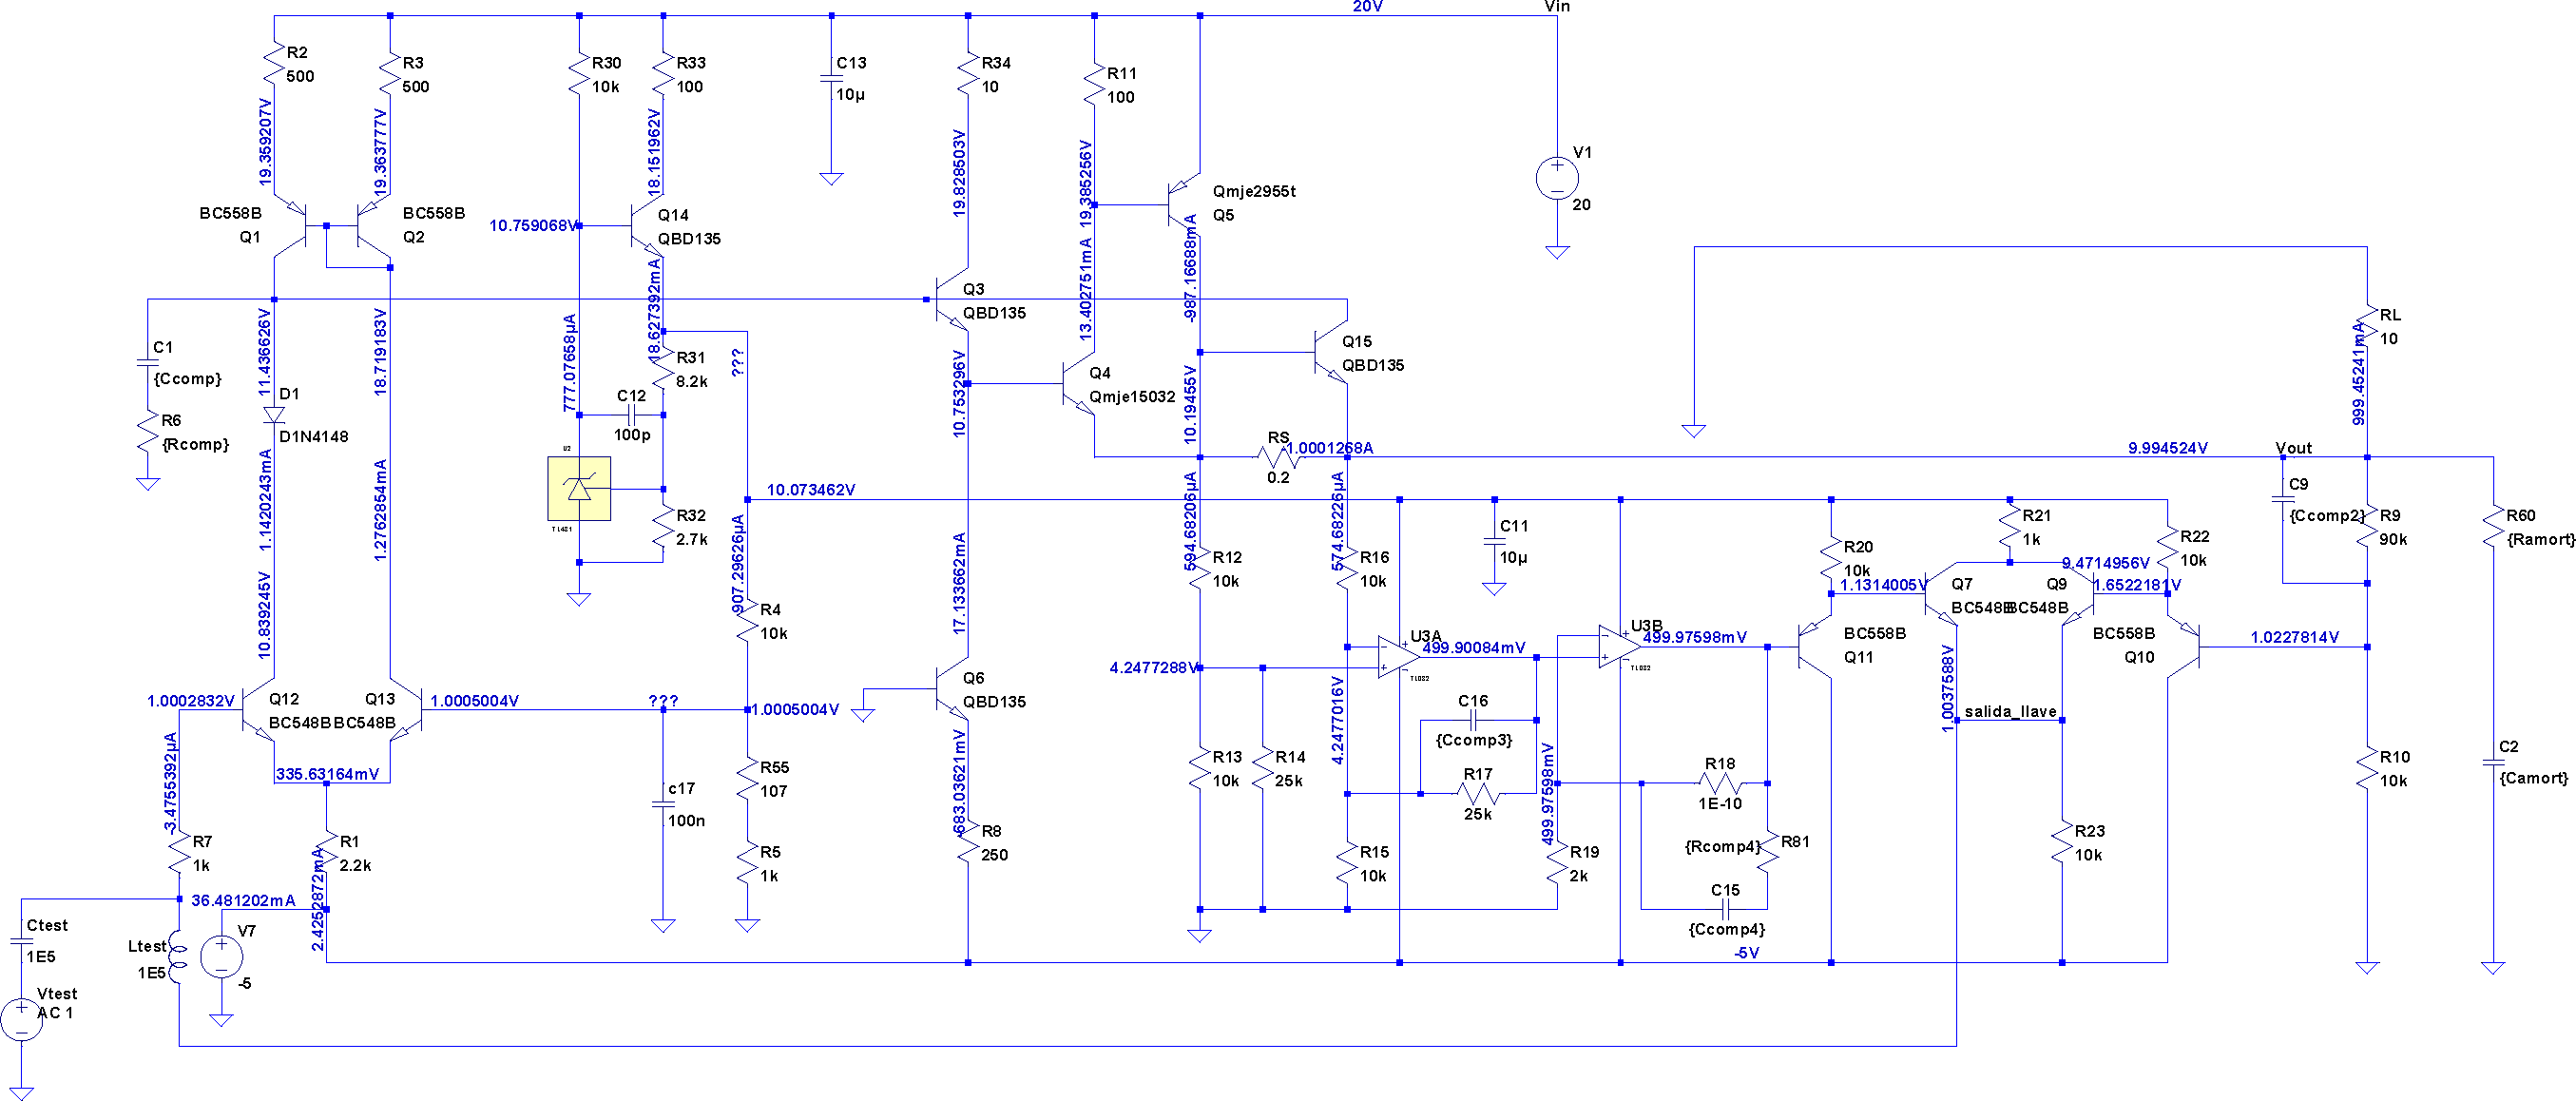
\includegraphics[width=1.2 \textwidth, angle=90]{./img/desarrollo/power_supply_LOOP.png}
\caption{\label{fig:fig_complete_circuit_loop}\footnotesize{Circuito utilizado para la obtención de la ganancia de lazo en función de la frecuencia.}}
\end{center}
\end{figure}

\clearpage

\begin{figure}[H] %htb
\begin{center}
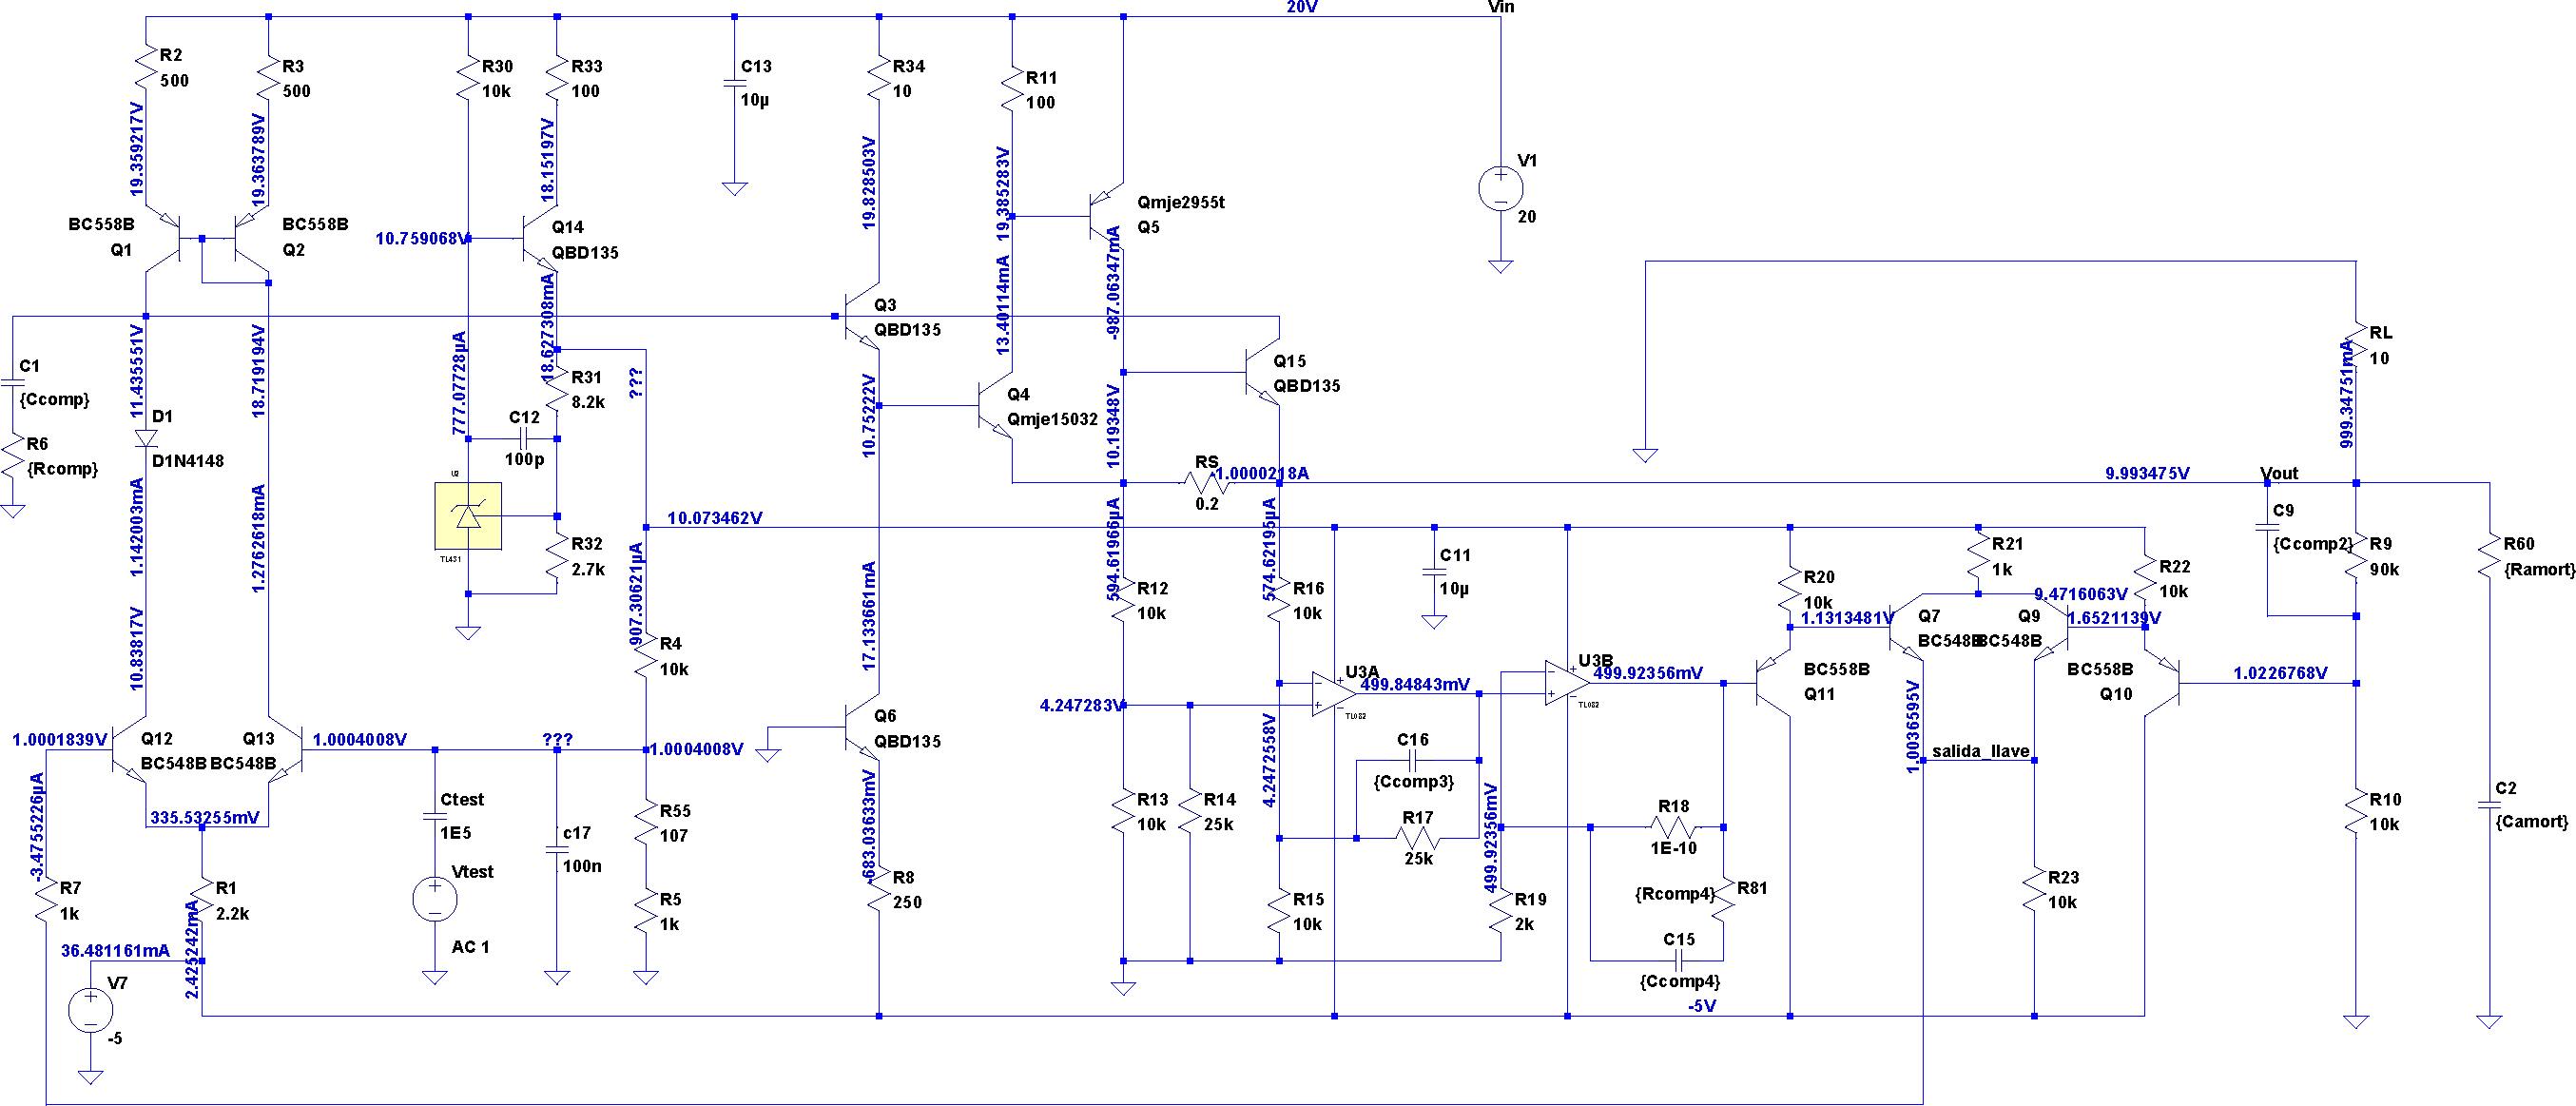
\includegraphics[width=1.2 \textwidth, angle=90]{./img/desarrollo/power_supply_RF.png}
\caption{\label{fig:fig_complete_circuit_rf}\footnotesize{Circuito utilizado para la obtención de la respuesta en frecuencia.}}
\end{center}
\end{figure}

\clearpage

\begin{figure}[H] %htb
\begin{center}
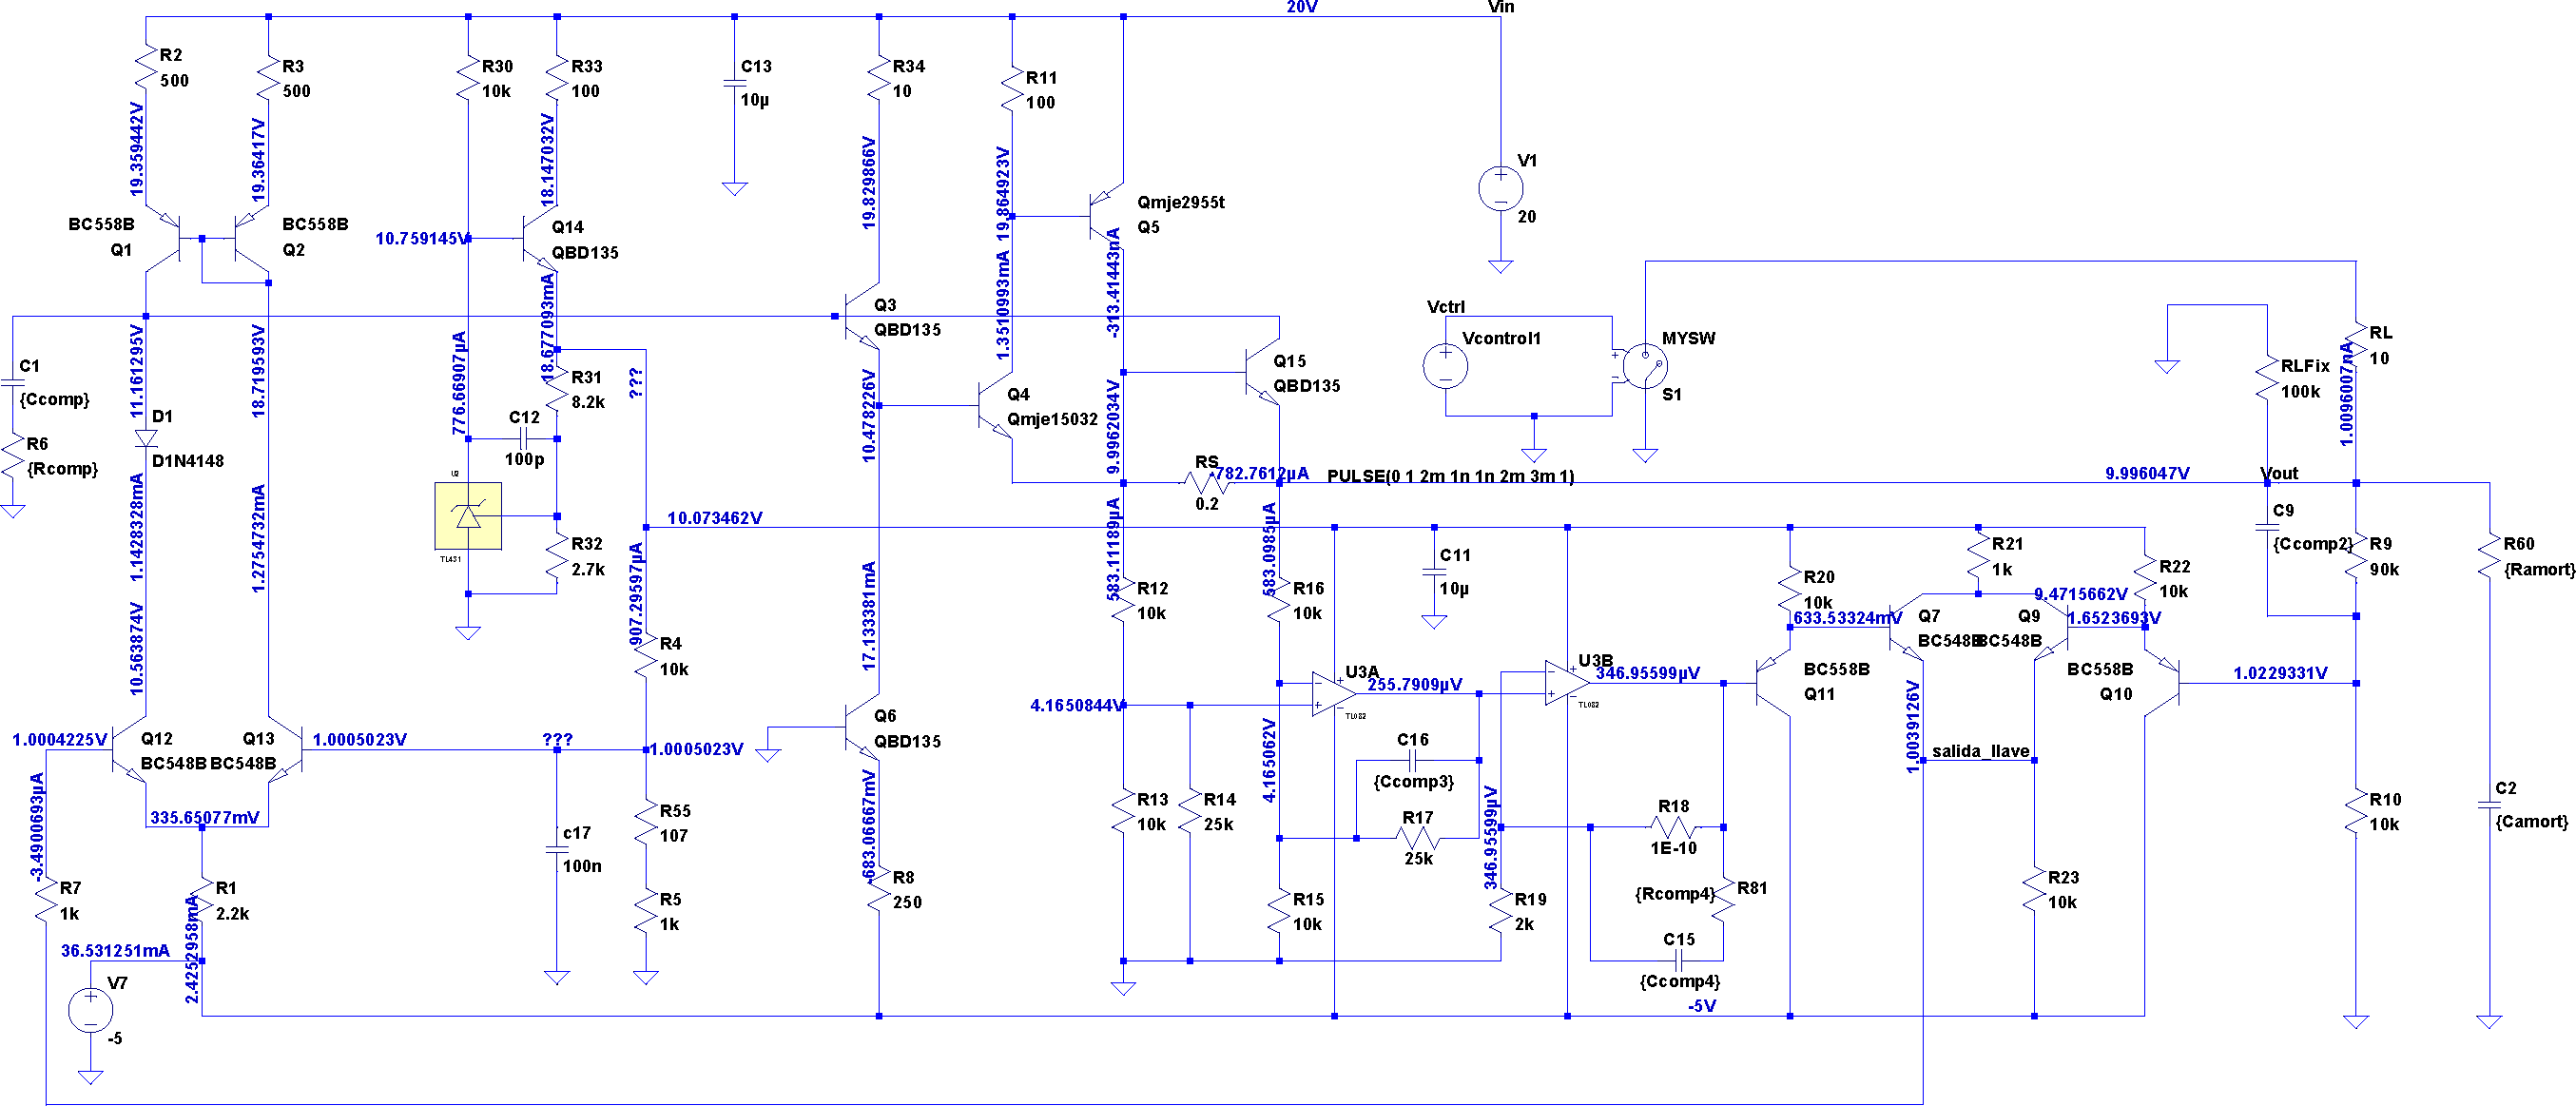
\includegraphics[width=1.2 \textwidth, angle=90]{./img/desarrollo/power_supply_STEP.png}
\caption{\label{fig:fig_complete_circuit_step}\footnotesize{Circuito utilizado para la obtención de la respuesta dinámica.}}
\end{center}
\end{figure}
\clearpage
%\\\\\\\\\\\\\\\\\\\\\\\\\\\

%\\\\\\\\\\\\\\\\\\\\\\\\\\\
\section{Análisis cualitativo}
\resetallcounters

\subsection{Secciones del circuito}


\normalfont

La topología del circuito corresponde a la de un típico amplificador de potencia de tres etapas realimentado, donde la \quotemarks{señal} a amplificar es una referencia de tensión, armada en torno a una referencia de tensión comercial, el \textbf{TL431}, la tensión de salida es muestreada y sumada a la entrada, formando un lazo de realimentación \textbf{serie-paralelo}, estabilizando la tensión de salida, el resultado de esta configuración es una fuente de tensión regulada. El circuito además posee un segundo lazo de realimentación, donde se muestrea la corriente de salida, se convierte a tensión y se suma a la entrada, formando un lazo de realimentación \textbf{serie-serie}, estabilizando la corriente de salida. El circuito trabaja con solo uno de los lazos de realimentación funcionando en un dado momento, el switcheo de uno a otro, se realiza en forma automática, con un subcircuito dedicado, según sea el estado de carga, el amplificador de potencia es el mismo en ambos lazos, solo cambia la red de realimentación. El circuito además cuenta con una limitación extra de corriente que actúa únicamente durante transitorios, además el circuito se encuentra compensado en frecuencia en ambos lazos (tema de la segunda parte del trabajo práctico).
En el circuito se pueden diferenciar claramente las secciones que se marcan en la figura~\figref{fig:fig_complete_circuit_secions}, las mismas son:


\begin{itemize}
\item Amplificador diferencial con caga activa: realiza la suma (resta) de la señal realimentada y provee amplificación.
\item Referencia de tensión: Provee una tensión estable de referencia de aproximadamente $1 \si[per-mode=symbol]{\volt}$ y además provee alimentación para algunas partes del circuito ($10 \si[per-mode=symbol]{\volt}$).
\item Seguidor con carga activa: Provee adaptación de impedancia entre la primera y la tercera etapa.
\item Par compuesto (Sziklai): Maneja la corriente de salida, presentando a la carga una muy baja impedancia y una alta impedancia a la segunda etapa.
\item Limitación de corriente simple: Formada solo por un transistor que limita durante transitorios, simplemente deriva corriente de la base del seguidor (segunda etapa).
\item Llave analógica: Hace el switcheo automático entre los lazos de tensión y corriente, es prácticamente transparente a fines prácticos.
\item Realimentación de tensión: Red de muestreo y realimentación de tensión (la mitad de la llave forma parte de la misma).
\item Realimentación de corriente: Red de muestreo y realimentación de corriente (la mitad de la llave forma parte de la misma).
\end{itemize}


\clearpage
%\\\\\\\\\\\\\\\\\\\\\\\\\\\

%\\\\\\\\\\\\\\\\\\\\\\\\\\\
\section{Punto de reposo}
\resetallcounters

Se hizo inicialmente un cálculo del punto de reposo en forma manual para la fuente de alimentación en regulación de tensión y de corriente, pero los valores obtenidos a pesar de ser lógicos diferían bastante respecto de la simulación, en particular, como es de esperarse, la etapa diferencial, por lo tanto se decidió utilizar los valores obtenidos de la simulación para los puntos de trabajo y los elementos del modelo de pequeña señal de cada dispositivo activo.
A continuación en los cuadros~\tableref{table:table_qpoint_voltage_regulation}~y~\tableref{table:table_qpoint_current_regulation} se resumen los valores obtenidos para todos los transistores en el caso de regulación de tensión ($R_{L}=100 \Omega$) y regulación de corriente ($R_{L}=0 \Omega$) respectivamente.



%% \noindent
%% \begin{center}
 
%%\begin{spacing}{1}  
\begin{table}[H]  %%\centering
    
    \setlength\arrayrulewidth{1.5pt}
    \arrayrulecolor{white}
    \def\clinecolor{\hhline{|>{\arrayrulecolor{white}}-%
    >{\arrayrulecolor{white}}|-|-|-|-|-|-|-|-|-|-|-|-|}}
\resizebox{0.85 \textwidth}{!}{% 
       
\begin{tabularx}{1 \textwidth}%
    {|
    >{\columncolor{white} \centering\arraybackslash}m{0.130\linewidth}
     |
    >{\columncolor{white} \centering\arraybackslash}m{0.065\linewidth}
     |
    >{\columncolor{white} \centering\arraybackslash}m{0.065\linewidth}
     |
    >{\columncolor{white} \centering\arraybackslash}m{0.065\linewidth}
     |
    >{\columncolor{white} \centering\arraybackslash}m{0.065\linewidth}
     |
    >{\columncolor{white} \centering\arraybackslash}m{0.065\linewidth} 
     |
    >{\columncolor{white} \centering\arraybackslash}m{0.065\linewidth}  
     |
    >{\columncolor{white} \centering\arraybackslash}m{0.065\linewidth}  
     |
    >{\columncolor{white} \centering\arraybackslash}m{0.065\linewidth} 
     |
    >{\columncolor{white} \centering\arraybackslash}m{0.065\linewidth}  
     |
    >{\columncolor{white} \centering\arraybackslash}m{0.065\linewidth} 
     |
    >{\columncolor{white} \centering\arraybackslash}m{0.065\linewidth} 
     |
    }
    \rowcolor{HeadersColor} \cellcolor{white} \thead{}  & \thead{Q1} & \thead{Q2} & \thead{Q3} & \thead{Q4} & \thead{Q5} & \thead{Q6} & \thead{Q9} & \thead{Q10} & \thead{Q12} & \thead{Q13} & \thead{Q14} \\
    
    \hhline{|-|-|-|-|-|-|-|-|-|-|-|-|}
    \rowcolor{gray!20} \cellcolor{LightPlum} $I_{C}$ [$mA$] & 1.28 & 1.26 & 17 & 3.93 & 16.7 & 17.1 & 0.603 &  0.837 & 1.15 & 1.27 & 18.5  \\
    \hhline{|-|-|-|-|-|-|-|-|-|-|-|-|}
    \rowcolor{gray!20} \cellcolor{LightPlum} $gm$ [$\frac{A}{V}$] & \num{4.89e-2} & \num{4.79e-2} & \num{6.58e-1} & \num{1.21e-1} & \num{7.43e-1} & \num{6.62e-1} & \num{2.32e-2} & \num{3.2e-2} & \num{4.39e-2} & \num{4.85e-2} & \num{7.15e-1}  \\
    \hhline{|-|-|-|-|-|-|-|-|-|-|-|-|}
    \rowcolor{gray!20} \cellcolor{LightPlum}  $r_{\pi}$ [$\Omega$] & 8.08 k & 5.74 k & 197 & 927 & 189 & 184 & 14.5 k & 10.1 k & 7.21 k & 8.12 k & 174  \\
    \hhline{|-|-|-|-|-|-|-|-|-|-|-|-|}
    \rowcolor{gray!20} \cellcolor{LightPlum} $r_{o}$ [$\Omega$] & 40.7 k & 28.9 k & 13.9 k & 10.5 k & 2.1 k & 13 k & 117 k & 50.9 k & 56 k & 63.5 k & 12.3 k  \\
    \hhline{|-|-|-|-|-|-|-|-|-|-|-|-|}
    \rowcolor{gray!20} \cellcolor{LightPlum} $\beta$ & 395 & 275 & 130 & 112 & 140 & 122 & 335 & 324 & 316 & 394 & 124  \\
    \hhline{|-|-|-|-|-|-|-|-|-|-|-|-|}          
    \end{tabularx}}
	\caption{\footnotesize{Elementos del modelo de pequeña señal de los transistores en regulación de tensión.}}
	\label{table:table_qpoint_voltage_regulation}
\end{table}
%%\end{spacing}

%% \end{center}


El par de transistores transistores $Q_{7}/Q_{11}$ no se considera por estar $Q_{7}$ cortado, lo mismo para el transistor $Q_{15}$, en el punto correspondiete se explica las razones y el funcionamiento del subcircuito.



%% \noindent
%% \begin{center}
 
%%\begin{spacing}{1}  
\begin{table}[H]  %%\centering
    
    \setlength\arrayrulewidth{1.5pt}
    \arrayrulecolor{white}
    \def\clinecolor{\hhline{|>{\arrayrulecolor{white}}-%
    >{\arrayrulecolor{white}}|-|-|-|-|-|-|-|-|-|-|-|-|}}
\resizebox{0.85 \textwidth}{!}{% 
       
\begin{tabularx}{1 \textwidth}%
    {|
    >{\columncolor{white} \centering\arraybackslash}m{0.130\linewidth}
     |
    >{\columncolor{white} \centering\arraybackslash}m{0.065\linewidth}
     |
    >{\columncolor{white} \centering\arraybackslash}m{0.065\linewidth}
     |
    >{\columncolor{white} \centering\arraybackslash}m{0.065\linewidth}
     |
    >{\columncolor{white} \centering\arraybackslash}m{0.065\linewidth}
     |
    >{\columncolor{white} \centering\arraybackslash}m{0.065\linewidth} 
     |
    >{\columncolor{white} \centering\arraybackslash}m{0.065\linewidth}  
     |
    >{\columncolor{white} \centering\arraybackslash}m{0.065\linewidth}  
     |
    >{\columncolor{white} \centering\arraybackslash}m{0.065\linewidth} 
     |
    >{\columncolor{white} \centering\arraybackslash}m{0.065\linewidth}  
     |
    >{\columncolor{white} \centering\arraybackslash}m{0.065\linewidth} 
     |
    >{\columncolor{white} \centering\arraybackslash}m{0.065\linewidth} 
     |
    }
    \rowcolor{HeadersColor} \cellcolor{white} \thead{}  & \thead{Q1} & \thead{Q2} & \thead{Q3} & \thead{Q4} & \thead{Q5} & \thead{Q6} & \thead{Q7} & \thead{Q11} & \thead{Q12} & \thead{Q13} & \thead{Q14} \\
    
    \hhline{|-|-|-|-|-|-|-|-|-|-|-|-|}
    \rowcolor{gray!20} \cellcolor{LightPlum} $I_{C}$ [$mA$] & 1.28 & 1.26 & 17.2 & 19.7 & 2040 & 17.1 & 0.603 & 0.837 & 1.15 & 1.27 & 18.5  \\
    \hhline{|-|-|-|-|-|-|-|-|-|-|-|-|}
    \rowcolor{gray!20} \cellcolor{LightPlum} $gm$ [$\frac{A}{V}$] & \num{4.9e-2} & \num{4.79e-2} & \num{6.64e-1} & \num{6.07e-1} & 54.3 & \num{6.62e-1} & \num{2.32e-2} & \num{3.2e-2} & \num{4.39e-2} & \num{4.85e-2} & \num{7.15e-1}  \\
    \hhline{|-|-|-|-|-|-|-|-|-|-|-|-|}
    \rowcolor{gray!20} \cellcolor{LightPlum}  $r_{\pi}$ [$\Omega$] & 8.32 k & 5.75 k & 197 & 186 & 2.11 & 183 & 14.5 k & 10.1 k & 7.21 k & 8.12 k & 174  \\
    \hhline{|-|-|-|-|-|-|-|-|-|-|-|-|}
    \rowcolor{gray!20} \cellcolor{LightPlum} $r_{o}$ [$\Omega$] & 41.8 k & 29 k & 13.9 k & 2.12 k & 17.9 k & 12.9 k & 117 k & 50.9 k & 56 k & 63.5 k & 12.3 k  \\
    \hhline{|-|-|-|-|-|-|-|-|-|-|-|-|}
    \rowcolor{gray!20} \cellcolor{LightPlum} $\beta$ & 407 & 275 & 131 & 113 & 115 & 121 & 335 & 324 & 316 & 394 & 124  \\
    \hhline{|-|-|-|-|-|-|-|-|-|-|-|-|}          
    \end{tabularx}}
	\caption{\footnotesize{Elementos del modelo de pequeña señal de los transistores en regulación de corriente.}}
	\label{table:table_qpoint_current_regulation}
\end{table}
%%\end{spacing}

%% \end{center}


El par de transistores transistores $Q_{9}/Q_{10}$ no se considera por estar $Q_{9}$ cortado, lo mismo para el transistor $Q_{15}$, ídem al caso anterior.
El diodo $D_{1}$ presenta una resistencia dinámica equivalente de $r_{d_{D_{1}}}=46.8 \Omega$ en ambos casos, también presenta una capacidad equivalente que no es considerada para el reposo (pero es importante en su funcionamiento dinámico).


Algo importante a observar es la perfecta inversión de los puntos de reposo de los pares de transistores $Q_{9}/Q_{10}$ y  $Q_{7}/Q_{11}$, sus puntos de reposo son idénticos al estar activos en el correspondiente lazo de realimentación, se explica en detalle mas adelante. El transistor  $Q_{15}$ solo conduce por breves períodos de tiempo al limitar picos de corriente, en estado estacionario siempre está cortado.



\clearpage
%\\\\\\\\\\\\\\\\\\\\\\\\\\\

%\\\\\\\\\\\\\\\\\\\\\\\\\\\
\section{Análisis de la ganancia a lazo abierto en regulación de tensión (bajas\textbackslash medias frecuencias)}
\resetallcounters
\subsection{Análisis de la ganancia de la etapa diferencial, $Q_{12}/Q_{13}$}

\subsubsection{Análisis de la fuente espejo}

\subsubsection{Ganancia de tensión}

\subsubsection{Resistencia de entrada}

\subsubsection{Resistencia de salida}


\subsection{Análisis de la ganancia de la etapa en seguidor por emisor, $Q_{3}$}

\subsubsection{Análisis de la fuente de corriente}

\subsubsection{Ganancia de tensión}

\subsubsection{Resistencia de entrada}

\subsubsection{Resistencia de salida}


\subsection{Análisis de la ganancia de la etapa del par compuesto (Sziklai) en seguidor por emisor, $Q_{4}/Q_{5}$}

\subsubsection{Ganancia de tensión}

\subsubsection{Resistencia de entrada}

\subsubsection{Resistencia de salida}


\clearpage
%\\\\\\\\\\\\\\\\\\\\\\\\\\\

%\\\\\\\\\\\\\\\\\\\\\\\\\\\
\section{Análisis del camino de ralimentación de tensión}
\resetallcounters

\label{section:switch_small_signal_begin}

\subsection{Análisis de etapa en seguidor por emisor, $Q_{10}$}

\subsubsection{Análisis de la ganancia de tensión}

Dado que este circuito no cumple la condición, $r_{o} \gg R_{E}$ no se puede usar la expresión aproximada $A_{v} \approx \frac{gm \cdot R_{E}}{1 + gm \cdot R_{E}}$, con lo que tenemos:

\begin{equation}
A_{v_{Q_{10}}} = \frac{1}{1 + \frac{r_{\pi_{10}}}{  \left(  \beta_{10} + 1 \right) \cdot \left(  R_{i_{B_{Q_{9}}}} \parallelresistors r_{o_{10}}  \right)  } }
\end{equation}

\begin{equation*}
A_{v_{Q_{10}}} = \frac{1}{1 + \frac{10.1 \si[per-mode=symbol]{\kilo\ohm}}{  \left(  324 + 1 \right) \cdot \left(  1.47 \si[per-mode=symbol]{\mega\ohm} \parallelresistors 50.9 \si[per-mode=symbol]{\kilo\ohm}  \right)  } } = 0.999
\end{equation*}


\subsubsection{Análisis de la resistencia de entrada}

Para calcular la  resistencia de entrada, vemos que no se cumple la condición $r_{o} \gg R_{E}$, con lo que la expresión aproximada, $ R_{i_{B_{Q_{3}}}} \approx r_{\pi_{3}} + \beta_{3} \cdot R_{E}$ no se puede usar.\\ \\

Tenemos entonces:

\begin{equation}
R_{i_{seguidor_{Q_{10}}}} = R_{i_{B_{Q_{10}}}} = r_{\pi_{10}} + \left( \beta_{10} + 1 \right) \cdot  \left(  R_{i_{seguidor_{Q_{9}}}} \parallelresistors R_{22}   \right)  \cdot \frac{  r_{o_{10}} }{  r_{o_{10}} + \left(  1.47 \si[per-mode=symbol]{\mega\ohm} \parallelresistors R_{22}   \right)  }
\end{equation}


\begin{equation*}
R_{i_{seguidor_{Q_{10}}}} = R_{i_{B_{Q_{10}}}} = 10.1 \si[per-mode=symbol]{\kilo\ohm} + \left( 324 + 1 \right) \cdot  \left(  R_{i_{seguidor_{Q_{9}}}} \parallelresistors 10 \si[per-mode=symbol]{\kilo\ohm}   \right)  \cdot \frac{  50.9 \si[per-mode=symbol]{\kilo\ohm} }{  50.9 \si[per-mode=symbol]{\kilo\ohm} + \left(  1.47 \si[per-mode=symbol]{\mega\ohm} \parallelresistors 10 \si[per-mode=symbol]{\kilo\ohm}   \right)  } = 2.7 \si[per-mode=symbol]{\mega\ohm}
\end{equation*}


\subsubsection{Análisis de la resistencia de salida}

\begin{equation}
R_{o_{seguidor_{Q_{10}}}} = r_{d_{10}} + \frac{   R_{10} \parallelresistors \left( R_{9} + \left[  R_{L} \parallelresistors \left( R_{S} + R_{o_{Sziklai}} \right) \right]  \right) }{\beta_{10}}  
\end{equation}


\begin{equation*}
R_{o_{seguidor_{Q_{10}}}} = 31.25 \si[per-mode=symbol]{\ohm} + \frac{   10 \si[per-mode=symbol]{\kilo\ohm} \parallelresistors \left( 10 \si[per-mode=symbol]{\kilo\ohm} + \left[  100 \si[per-mode=symbol]{\ohm} \parallelresistors \left( 0.2 \si[per-mode=symbol]{\ohm} + 114.11 \si[per-mode=symbol]{\milli\ohm} \right) \right]  \right) }{324} = 46.68 \si[per-mode=symbol]{\ohm}
\end{equation*}


\subsection{Análisis de etapa en seguidor por emisor, $Q_{9}$}



\subsubsection{Análisis de la ganancia de tensión}

\begin{equation}
A_{v_{Q_{9}}} = \frac{1}{1 + \frac{r_{\pi_{9}}}{  \left(  \beta_{9} + 1 \right) \cdot \left(  R_{23} \parallelresistors \left(  R_{7} + r_{\pi_{12}} \right) \parallelresistors r_{o_{9}}  \right)  } }
\end{equation}


\begin{equation*}
A_{v_{Q_{9}}} = \frac{1}{1 + \frac{ 14.5 \si[per-mode=symbol]{\kilo\ohm} }{  \left(  335 + 1 \right) \cdot \left(  10 \si[per-mode=symbol]{\kilo\ohm} \parallelresistors \left(  1 \si[per-mode=symbol]{\kilo\ohm} + 7.21 \si[per-mode=symbol]{\kilo\ohm} \right) \parallelresistors 117 \si[per-mode=symbol]{\kilo\ohm}  \right)  } } = 0.99
\end{equation*}


\subsubsection{Análisis de la resistencia de entrada}

\begin{equation}
R_{i_{seguidor_{Q_{9}}}} = R_{i_{B_{Q_{9}}}} = r_{\pi_{9}} + \left( \beta_{9} + 1 \right) \cdot  \left[  R_{23} \parallelresistors \left(  R_{7} + r_{\pi_{12}} \right)   \right]  \cdot \frac{  r_{o_{9}} }{  r_{o_{9}} + \left[  R_{23} \parallelresistors \left(  R_{7} + r_{\pi_{12}} \right)   \right]  }
\end{equation}


\begin{equation*}
R_{i_{seguidor_{Q_{9}}}} = R_{i_{B_{Q_{9}}}} = 14.5 \si[per-mode=symbol]{\kilo\ohm} + \left( 335 + 1 \right) \cdot  \left[  10 \si[per-mode=symbol]{\kilo\ohm} \parallelresistors \left(  1 \si[per-mode=symbol]{\kilo\ohm} + 7.21 \si[per-mode=symbol]{\kilo\ohm} \right)   \right]  \cdot \frac{  117 \si[per-mode=symbol]{\kilo\ohm} }{  117 \si[per-mode=symbol]{\kilo\ohm} + \left[  10 \si[per-mode=symbol]{\kilo\ohm} \parallelresistors \left(  1 \si[per-mode=symbol]{\kilo\ohm} + 7.21 \si[per-mode=symbol]{\kilo\ohm} \right)   \right]  } = 1.47 \si[per-mode=symbol]{\mega\ohm}
\end{equation*}

\subsubsection{Análisis de la resistencia de salida}

\begin{equation}
R_{o_{seguidor_{Q_{9}}}} = r_{d_{9}} + \frac{R_{o_{seguidor_{Q_{10}}}}}{\beta_{9}}  
\end{equation}

\begin{equation*}
R_{o_{seguidor_{Q_{9}}}} = 43.10 \si[per-mode=symbol]{\ohm} + \frac{46.68 \si[per-mode=symbol]{\ohm}}{335} = 43.24 \si[per-mode=symbol]{\ohm} 
\end{equation*}



\label{section:switch_small_signal_end}


\subsection{Análisis del divisor resistivo de realimentación $R_{9}/R_{10}$}

Dado el valor de $R_{i_{seguidor_{Q_{10}}}} = 2.7 \si[per-mode=symbol]{\mega\ohm}$, y el valor de $R_{9}$ y $R_{10}$, se puede asumir que el mismo no está cargado, por lo que su transferencia, será entonces:

\begin{equation}
T_{D_{R_{9}-R_{10}}} = \frac{R_{10}}{R_{9} + R_{10}}
\end{equation}



\subsection{Transferencia del realimentador \textbf{serie-paralelo}}

Dado que el divisor resistivo tiene su transferencia ideal al no estar cargado, tenemos en el camino de realimentación de tensión solo este divisor y la ganancia en cascada de ambos seguidores, la llamamos ganancia de la llave, cuyo valor es:


\begin{equation}
A_{v_{llave}} = A_{v_{Q_{10}}} \cdot A_{v_{Q_{9}}}
\end{equation}

\begin{equation*}
A_{v_{llave}} = 0.999 \times 0.99 \approx 0.99
\end{equation*}


La resistencia de salida de la llave, será la vista hacia la salida del seguidor basado en $Q_{9}$, la misma se ve en paralelo con $R_{23}$, tenemos entonces:

\begin{equation}
R_{o_{llave}} = R_{o_{seguidor_{Q_{9}}}} \parallelresistors R_{23}
\end{equation}

\begin{equation*}
R_{o_{llave}} = 43.24 \si[per-mode=symbol]{\ohm} \parallelresistors 10 \si[per-mode=symbol]{\kilo\ohm} = 43.05 \si[per-mode=symbol]{\ohm}
\end{equation*}


\subsection{Cálculo de la ganancia de lazo para el lazo de tensión}

\label{section:voltage_loop_justification}


En la figura~\figref{fig:fig_voltage_loop_1}, puede verse el esquema de la fuente de alimentación como circuito realimentado, puede verse que se trata de realimentación \textbf{serie-paralelo}, que como es de esperarse estabiliza la tensión de salida.

\begin{figure}[H] %htb
\begin{center}
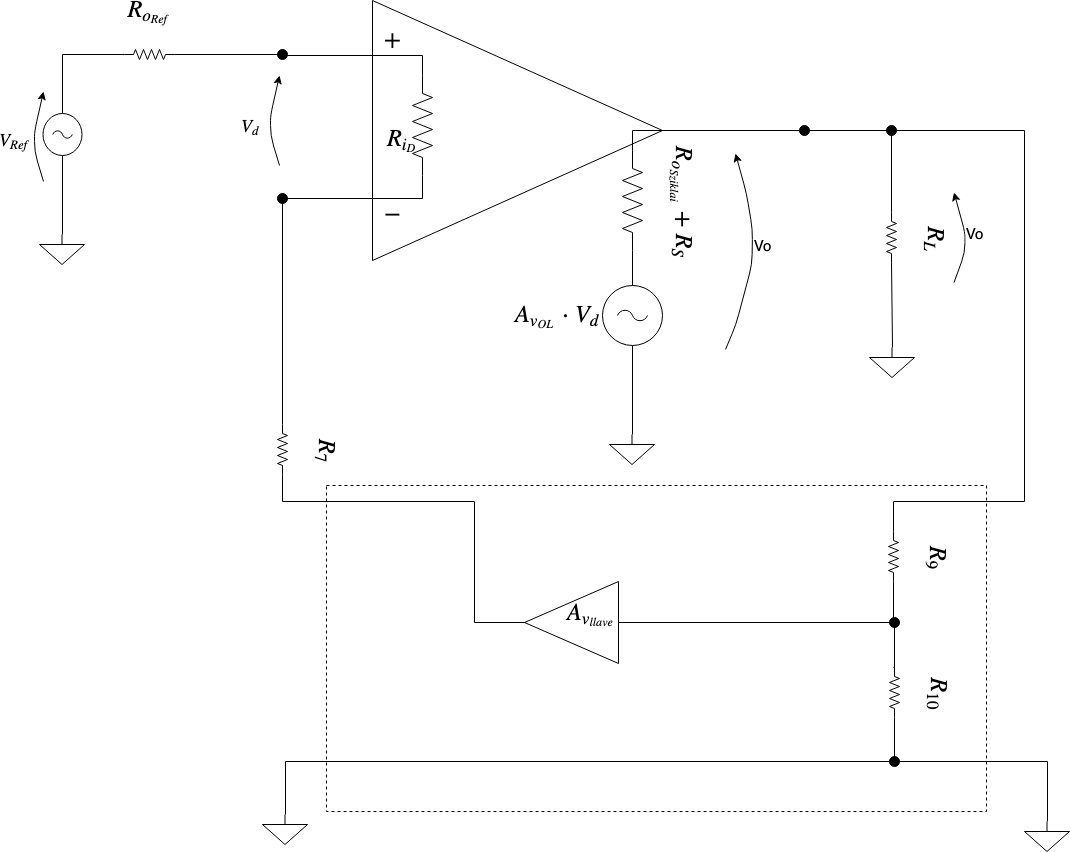
\includegraphics[width=0.9 \textwidth, angle=0]{./img/voltage_loop/VOLTAGE_LOOP_1.png}
\caption{\label{fig:fig_voltage_loop_1}\footnotesize{Esquema de la fuente de alimentación como circuito realimentado}}
\end{center}
\end{figure}

Aplicando parámetros \textbf{h} al realimentador, y reordenando el circuito para llevar el realimentador a su forma ideal, se obtiene lo que se muestra en la figura~\figref{fig:fig_voltage_loop_2}


\begin{figure}[H] %htb
\begin{center}
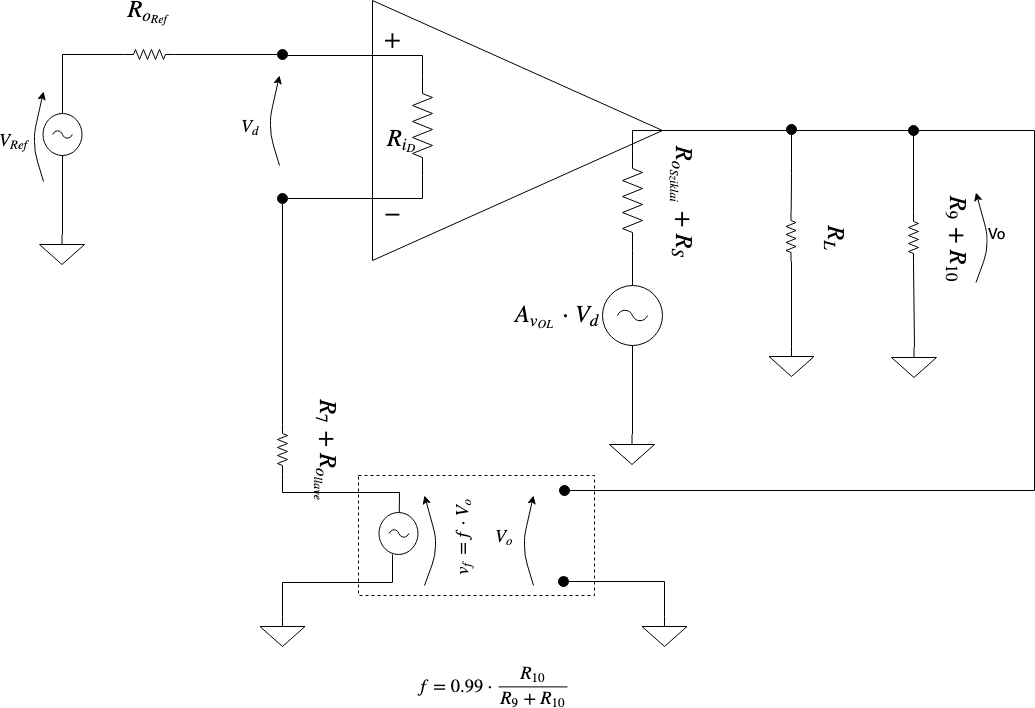
\includegraphics[width=0.9 \textwidth, angle=0]{./img/voltage_loop/VOLTAGE_LOOP_2.png}
\caption{\label{fig:fig_voltage_loop_2}\footnotesize{Aplicando parámetros \textbf{h} al realimentador}}
\end{center}
\end{figure}

\begin{equation}
f = 0.99 \times \frac{R_{10}}{R{9} + R{10}}
\end{equation}



Finalmente tenemos para la ganancia de tensión a lazo cerrado:


\begin{equation}
A = \frac{a}{1 + a \cdot f}
\end{equation}

\begin{equation*}
\boxed{ A = \frac{2382.03}{1 + 2382.03 \times 0.99 \times \frac{R_{10}}{R{9} + R{10}}} \approx 1.01 \times \left(  1 + \frac{R_{9}}{R{10}} \right) }
\end{equation*}

\subsection{Cálculo de la tensión de salida a lazo cerrado}


Para la tensión de salida, asumiendo una tensión de referencia de exactamente $1 \si[per-mode=symbol]{\volt}$:

\begin{equation*}
\boxed{ V{o} = A \cdot V_{Ref} = 1.01 \si[per-mode=symbol]{\volt} \times \left(  1 + \frac{R_{9}}{R{10}} \right) }
\end{equation*}



\subsection{Cálculo de la resistencia de salida a lazo abierto}


La resistencia de la fuente en el nodo de salida a lazo abierto será:

\begin{equation}
R_{o_{OL}} \approx R_{o_{Sziklai}} + R_{S}
\end{equation}


\subsection{Cálculo de la resistencia de salida a lazo cerrado}


Se tendrá entonces a lazo cerrado

\begin{equation}
R_{o} =  \frac{R_{o_{Sziklai}} + R_{S}}{1 + a \cdot f} 
\end{equation}


\begin{equation}
\boxed{R_{o} = \frac{114.11 \si[per-mode=symbol]{\milli\ohm} + 0.2 \si[per-mode=symbol]{\ohm}}{1 + 2382.03 \times 0.99 \times \frac{R_{10}}{R{9} + R{10}}} = \frac{314.11 \si[per-mode=symbol]{\milli\ohm}}{1 + 2358.21 \times \frac{R_{10}}{R{9} + R_{10}}} \approx 133.20 \si[per-mode=symbol]{\micro\ohm} \times \left(  1 + \frac{R_{9}}{R{10}} \right) }
\end{equation}

El valor de la misma depende de la realimentación como era de esperar, (también de la ganancia de lazo, esta no es estabilizada). Para el caso de $R_{9} = 10 \si[per-mode=symbol]{\kilo\ohm}$ tenemos:

\begin{equation*}
R_{o_{10k}} = 266.4 \si[per-mode=symbol]{\micro\ohm}
\end{equation*}







\clearpage
%\\\\\\\\\\\\\\\\\\\\\\\\\\\


%\\\\\\\\\\\\\\\\\\\\\\\\\\\
\section{Observaciones y conclusiones}
\resetallcounters

\subsection{Observaciones y conclusiones}

Cuando empezamos el desarrollo del trabajo práctico intentamos desarrollarlo como si diseñáramos la compensación desde cero, a pesar de que las redes que concluimos que serían necesarias coincidían en la localización con las existentes en el diseño, nos encontramos que el cálculo de los valores requería un desarrollo teórico extenso y una validación iterativa por simulación que se hacia muy complicada en el tiempo disponible, no obstante este primer intento nos sirvió para entender que involucra el diseño de una compensación. \\
Otra cosa en el desarrollo del análisis por simulación es que nos costó un poco en algunos casos ver porque un valor es mejor que otro, al menos por lo que se podía ver en las simulaciones, eso puede ser porque faltan casos que simular, pero ya era bastante extenso como para hacer mas simulaciones. \\
Finalmente, viendo lo justa que queda la compensación para algunos casos, llegamos a la conclusión que sería necesario un análisis por el \textbf{método de Monte Carlo} para garantizar la estabilidad frente a las variaciones de los valores de los componentes, pero nuevamente, el análisis sería demasiado extenso, especialmente dado el tiempo que una simulación estadística puede tomar.
\cleardoublepage
%\\\\\\\\\\\\\\\\\\\\\\\\\\\

%\\\\\\\\\\\\\\\\\\\\\\\\\\\
%Reinicio la cuenta y seteo el estilo de headers y footers.
\pagestyle{bibliostyle}
%\\\\\\\\\\\\\\\\\\\\\\\\\\\

%\\\\\\\\\\\\\\\\\\\\\\\\\\\
\section{Bibliografía}
\resetallcounters

\begin{thebibliography}{9}




\bibitem{Gray_Meyer3}
\Needspace*{7\baselineskip}
\emph{Analysis and Design of Analog Integrated Circuits (3\textsuperscript{rd} Edition)}\\
Author: Paul R. Gray\\
Author: Robert G. Meyer\\
Publisher: John Wiley \& Sons, Inc.; 3\textsuperscript{rd} Edition (Janury 15, 1993)\\
Copyright: \textcopyright \space 1993, John Wiley \& Sons, Inc.\\
ISBN 10: 0471574953\\
Website: \weblink{http://www.wiley.com/WileyCDA/WileyTitle/productCd-EHEP000220.html}{Analysis and Design of Analog Integrated Circuits (3\textsuperscript{rd} Edition)}\\




\bibitem{Gray_Meyer4}
\Needspace*{10\baselineskip}
\emph{Analysis and Design of Analog Integrated Circuits (4\textsuperscript{th} Edition)}\\
Author: Paul R. Gray\\
Author: Paul J. Hurst\\
Author: Stephen H. Lewis\\
Author: Robert G. Meyer\\
Publisher: John Wiley \& Sons, Inc.; 4\textsuperscript{th} Edition (2001)\\
Copyright: \textcopyright \space 2001, John Wiley \& Sons, Inc.\\
ISBN 10: 0471321680\\
ISBN 13: 9780471321682\\
Website: \weblink{http://www.wiley.com/WileyCDA/WileyTitle/productCd-EHEP000220.html}{Analysis and Design of Analog Integrated Circuits (4\textsuperscript{th} Edition)}\\




\bibitem{Gray_Meyer5}
\Needspace*{10\baselineskip}
\emph{Analysis and Design of Analog Integrated Circuits (5\textsuperscript{th} Edition)}\\
Author: Paul R. Gray\\
Author: Paul J. Hurst\\
Author: Stephen H. Lewis\\
Author: Robert G. Meyer\\
Publisher: John Wiley \& Sons, Inc.; 5\textsuperscript{th} Edition (2009)\\
Copyright: \textcopyright \space 2001, John Wiley \& Sons, Inc.\\
ISBN 10: 0470245999\\
ISBN 13: 9780470245996\\
Website: \weblink{https://www.wiley.com/en-ar/Analysis+and+Design+of+Analog+Integrated+Circuits\%2C+5th+Edition-p-9780470245996}{Analysis and Design of Analog Integrated Circuits (5\textsuperscript{th} Edition)}\\



\bibitem{Sedra_Smith_ESP4}
\Needspace*{9\baselineskip}
\emph{Circuitos microelectrónicos (4\textsuperscript{ta} Edición) español}\\
Author: Adel. S. Sedra\\
Author: Kenneth C. Smith\\
Publisher: Oxford, University press; 4\textsuperscript{ta} Edición (2001)\\
Copyright: \textcopyright \space 1999, Oxford, University press México.\\
Original Copyright: \textcopyright \space 1998, 1991, 1987, 1982, Oxford, University press Inc.\\
ISBN 10: 01951166310\\
Website: \weblink{http://www.oup.com/us/companion.websites/0195142519/}{Circuitos microelectrónicos (4\textsuperscript{ta} Edición) español}\\




\bibitem{Sedra_Smith_ENG5}
\Needspace*{8\baselineskip}
\emph{Microelectronic circuits (5\textsuperscript{th} Edition)}\\
Author: Adel. S. Sedra\\
Author: Kenneth C. Smith\\
Publisher: Oxford, University press; 5\textsuperscript{th} Edition (2004)\\
Copyright: \textcopyright \space 2004, 1998, 1991, 1987, 1982, Oxford, University press Inc.\\
ISBN 10: 0195142527\\
Website: \weblink{http://www.oup.com/us/companion.websites/0195142519/}{Microelectronic circuits (5\textsuperscript{th} Edition)}\\





\end{thebibliography}
\cleardoublepage
%\\\\\\\\\\\\\\\\\\\\\\\\\\\

\appendix

\appendixpage
\addappheadtotoc

%\\\\\\\\\\\\\\\\\\\\\\\\\\\
%Seteo el stilo de headers y footers.
\pagestyle{codestyle}
%\\\\\\\\\\\\\\\\\\\\\\\\\\\


%\\\\\\\\\\\\\\\\\\\\\\\\\\\
%Seteo el stilo de headers y footers.
\pagestyle{codestyle}
%\\\\\\\\\\\\\\\\\\\\\\\\\\\

%\\\\\\\\\\\\\\\\\\\\\\\\\\\
%\section{Salidas de las simulaciones en \spice}
%\resetallcounters
%%*********************************************
\subsection{Consideraciones para los archivos de salida (archivos \textbf{\quotemarks{.out})}}
\thispagestyle{codeconsstyle}
\renewcommand{\themark}{Consideraciones para los archivos de salida (archivos \textbf{\quotemarks{.out}})}

El siguiente apéndice contiene los archivos \textbf{\quotemarks{.out}} completos producidos por las simulaciones en \spice, los mismos son transcritos completos y fueron producidos indicando que se incluya información detallada de polarización de los dispositivos semiconductores. La presentación de los archivos en el informe se hizo directamente desde los mismos hacia \LaTeX\space usando el paquete \textbf{\quotemarks{listingsutf8}}~\citelink{The_ListingsUTF8_Package}, que es una extensión con soporte para \textbf{UTF8} del paquete \textbf{\quotemarks{listings}}~\citelink{The_Listings_Package}, este paquete produce una salida formateada y con coloreado del contenido de los archivos y también permite el agregado de números de líneas y otros agregados. 
 

\clearpage
%*********************************************

%******************************************************************************************
\lstset{language=,numbers=left,xleftmargin=1em,stepnumber=1}

\lstset{showspaces=false}
\lstset{showstringspaces=false}

\lstset{backgroundcolor=\color{white},rulecolor=\color{blue}}
\lstset{basicstyle=\ttfamily\color{DarkBlue}}

%\lstset{keywordstyle=[1]\ttfamily\color{red}\bfseries}
%\lstset{keywordstyle=[2]\ttfamily\color{LightSkyBlue}}
%\lstset{keywordstyle=[3]\ttfamily\bfseries\color{Plum}}
%\lstset{keywordstyle=[4]\ttfamily\bfseries\color{Chocolate}}

%\lstset{identifierstyle=\ttfamily\color{black}}
%\lstset{commentstyle=\ttfamily\color{Aluminium4}\textit}
%\lstset{stringstyle=\ttfamily\color{purple}\upshape}
\lstset{tabsize=4}

\lstset{numberstyle=\ttfamily\color{Deeppurple}\upshape}
\lstset{numbersep=5pt}

\lstset{inputencoding=utf8/latin1}

%******************************************************************************************

\subsection{Salida de la simulación para la distorsión de salida con $R_{SS}$ desacoplada}

%*********************************************
\subsubsection{\quotefile{Distorsion\_wo\_Rss.out}}
\label{OUT_FILE_DIST_WO_RSS}
Simulación paramétrica en amplitud para la entrada del amplificador con $R_{SS}$ desacoplada.\\

\begin{flushleft}
\filebox{A continuación se muestra el archivo \textcolor{DarkBlue}{\quotefile{Distorsion\_wo\_Rss.out}}:}{Aluminium2}
\end{flushleft}

%\fontencoding{T1}
\fontseries{m}
\fontsize{5pt}{6pt}
\selectfont

\lstinputlisting{./sim_outs/Excursion_sin_Rss_m.out}

\normalfont
\normalsize
\selectfont

%*********************************************


\clearpage


%******************************************************************************************

\subsection{Salida de la simulación para la distorsión de salida con $R_{SS}$ sin desacoplar}

%*********************************************
\subsubsection{\quotefile{Distorsion\_w\_Rss.out}}
\label{OUT_FILE_DIST_W_RSS}
Simulación paramétrica en amplitud para la entrada del amplificador con $R_{SS}$ sin desacoplar.\\

\begin{flushleft}
\filebox{A continuación se muestra el archivo \textcolor{DarkBlue}{\quotefile{Distorsion\_w\_Rss.out}}:}{Aluminium2}
\end{flushleft}

%\fontencoding{T1}
\fontseries{m}
\fontsize{5pt}{6pt}
\selectfont

\lstinputlisting{./sim_outs/Excursion_con_Rss_m.out}

\normalfont
\normalsize
\selectfont

%*********************************************

%\cleardoublepage
%\\\\\\\\\\\\\\\\\\\\\\\\\\\

%\\\\\\\\\\\\\\\\\\\\\\\\\\\
%Seteo el stilo de headers y footers.
\pagestyle{allpages}
%\\\\\\\\\\\\\\\\\\\\\\\\\\\

%\\\\\\\\\\\\\\\\\\\\\\\\\\\
\section{Hojas de datos}
\resetallcounters


%*********************************************

\subsection{TL431}
\label{datasheet_TL431}
\emph{\textbf{TL431}}\\
\emph{Adjustable precision shunt regulator}\\
\vspace{5pt}
Manufacturer page:	\weblink{http://www.ti.com/product/TL431}{http://www.ti.com/product/TL431}\\

Manufacturer Datasheet:	\weblink{http://www.ti.com/lit/gpn/tl431}{http://www.ti.com/lit/gpn/tl431}\\


\subsection{TL082}
\label{datasheet_TL082}
\emph{\textbf{TL082}}\\
\emph{Dual High Slew Rate JFET-Input Operational Amplifier}\\
\vspace{5pt}
Manufacturer page:	\weblink{http://www.ti.com/product/TL082?keyMatch=TL082}{http://www.ti.com/product/TL082?keyMatch=TL082}\\

Manufacturer Datasheet:	\weblink{http://www.ti.com/lit/gpn/tl082}{http://www.ti.com/lit/gpn/tl082}\\


\subsection{BC548}
\label{datasheet_BC548}
\emph{\textbf{BC548}}\\
\emph{NPN Epitaxial Silicon Transistor}\\
\vspace{5pt}
Manufacturer page:	\weblink{https://www.onsemi.com/PowerSolutions/product.do?id=BC548}{https://www.onsemi.com/PowerSolutions/product.do?id=BC548}\\

Manufacturer Datasheet:	\weblink{https://www.onsemi.com/pub/Collateral/BC550-D.pdf}{https://www.onsemi.com/pub/Collateral/BC550-D.pdf}\\


\subsection{BC558}
\label{datasheet_BC558}
\emph{\textbf{BC558}}\\
\emph{PNP Bipolar Transistor}\\
\vspace{5pt}
Manufacturer page:	\weblink{https://www.onsemi.com/PowerSolutions/product.do?id=BC558B}{https://www.onsemi.com/PowerSolutions/product.do?id=BC558B}\\

Manufacturer Datasheet:	\weblink{https://www.onsemi.com/pub/Collateral/BC556B-D.PDF}{https://www.onsemi.com/pub/Collateral/BC556B-D.PDF}\\

\clearpage


\subsection{BD137}
\label{datasheet_BD137}
\emph{\textbf{BD137}}\\
\emph{$1.5 \si[per-mode=symbol]{\ampere}$, $60 \si[per-mode=symbol]{\volt}$ NPN Bipolar Power Transistor}\\
\vspace{5pt}
Manufacturer page:	\weblink{https://www.onsemi.com/PowerSolutions/product.do?id=BD137}{https://www.onsemi.com/PowerSolutions/product.do?id=BD137}\\

Manufacturer Datasheet:	\weblink{https://www.onsemi.com/pub/Collateral/BD135-D.PDF}{https://www.onsemi.com/pub/Collateral/BD135-D.PDF}\\


\subsection{MJE15032}
\label{datasheet_MJE15032}
\emph{\textbf{MJE15032}}\\
\emph{Bipolar Transistor, NPN, $250 \si[per-mode=symbol]{\volt}$, $8.0 \si[per-mode=symbol]{\ampere}$}\\
\vspace{5pt}
Manufacturer page:	\weblink{https://www.onsemi.com/PowerSolutions/product.do?id=MJE15032}{https://www.onsemi.com/PowerSolutions/product.do?id=MJE15032}\\

Manufacturer Datasheet:	\weblink{https://www.onsemi.com/pub/Collateral/MJE15032-D.PDF}{https://www.onsemi.com/pub/Collateral/MJE15032-D.PDF}\\


\subsection{MJE2955}
\label{datasheet_MJE2955}
\emph{\textbf{MJE2955}}\\
\emph{Bipolar Power Transistor, PNP, $10 \si[per-mode=symbol]{\ampere}$, $60 \si[per-mode=symbol]{\volt}$, $75 \si[per-mode=symbol]{\watt}$}\\
\vspace{5pt}
Manufacturer page:	\weblink{https://www.onsemi.com/PowerSolutions/product.do?id=MJE2955T}{https://www.onsemi.com/PowerSolutions/product.do?id=MJE2955T}\\

Manufacturer Datasheet:	\weblink{https://www.onsemi.com/pub/Collateral/MJE2955T-D.PDF}{hhttps://www.onsemi.com/pub/Collateral/MJE2955T-D.PDF}\\


\subsection{Metal film resistor}
\label{datasheet_METALFILMRESISTOR}
\emph{\textbf{Metal film resistor}}\\
\emph{Metal film resistor}\\
\vspace{5pt}
Manufacturer page:	\weblink{https://www.vishay.com/resistors-fixed/metal-film/tab/doclibrary/}{https://www.vishay.com/resistors-fixed/metal-film/tab/doclibrary/}\\



\subsection{Carbon film resistor}
\label{datasheet_CARBONFILMRESISTOR}
\emph{\textbf{Carbon film resistor}}\\
\emph{Carbon film resistor}\\
\vspace{5pt}
Manufacturer page:	\weblink{http://www.vishay.com/resistors-fixed/carbon-film/tab/doclibrary/}{http://www.vishay.com/resistors-fixed/carbon-film/tab/doclibrary/}\\


\clearpage


\subsection{Ceramic capacitor}
\label{datasheet_CERAMIC_CAPACITOR}
\emph{\textbf{Ceramic capacitor}}\\
\emph{Ceramic disk capacitor}\\
\vspace{5pt}
Manufacturer page:	\weblink{https://www.vishay.com/capacitors/ceramic/disc/}{https://www.vishay.com/capacitors/ceramic/disc/}\\


\subsection{Electrolitic Aluminum capacitor}
\label{datasheet_ELECTROLITIC_CAPACITOR}
\emph{\textbf{Electrolitic capacitor}}\\
\emph{Electrolitic aluminum capacitor}\\
\vspace{5pt}
Manufacturer page:	\weblink{https://www.vishay.com/capacitors/aluminum/}{https://www.vishay.com/capacitors/aluminum/}\\









\cleardoublepage
%\\\\\\\\\\\\\\\\\\\\\\\\\\\


\end{document}
